% Options for packages loaded elsewhere
\PassOptionsToPackage{unicode}{hyperref}
\PassOptionsToPackage{hyphens}{url}
%
\documentclass[
]{book}
\usepackage{amsmath,amssymb}
\usepackage{lmodern}
\usepackage{iftex}
\ifPDFTeX
  \usepackage[T1]{fontenc}
  \usepackage[utf8]{inputenc}
  \usepackage{textcomp} % provide euro and other symbols
\else % if luatex or xetex
  \usepackage{unicode-math}
  \defaultfontfeatures{Scale=MatchLowercase}
  \defaultfontfeatures[\rmfamily]{Ligatures=TeX,Scale=1}
\fi
% Use upquote if available, for straight quotes in verbatim environments
\IfFileExists{upquote.sty}{\usepackage{upquote}}{}
\IfFileExists{microtype.sty}{% use microtype if available
  \usepackage[]{microtype}
  \UseMicrotypeSet[protrusion]{basicmath} % disable protrusion for tt fonts
}{}
\makeatletter
\@ifundefined{KOMAClassName}{% if non-KOMA class
  \IfFileExists{parskip.sty}{%
    \usepackage{parskip}
  }{% else
    \setlength{\parindent}{0pt}
    \setlength{\parskip}{6pt plus 2pt minus 1pt}}
}{% if KOMA class
  \KOMAoptions{parskip=half}}
\makeatother
\usepackage{xcolor}
\IfFileExists{xurl.sty}{\usepackage{xurl}}{} % add URL line breaks if available
\IfFileExists{bookmark.sty}{\usepackage{bookmark}}{\usepackage{hyperref}}
\hypersetup{
  pdftitle={Statistics Primer},
  pdfauthor={Aaron McMurray},
  hidelinks,
  pdfcreator={LaTeX via pandoc}}
\urlstyle{same} % disable monospaced font for URLs
\usepackage{longtable,booktabs,array}
\usepackage{calc} % for calculating minipage widths
% Correct order of tables after \paragraph or \subparagraph
\usepackage{etoolbox}
\makeatletter
\patchcmd\longtable{\par}{\if@noskipsec\mbox{}\fi\par}{}{}
\makeatother
% Allow footnotes in longtable head/foot
\IfFileExists{footnotehyper.sty}{\usepackage{footnotehyper}}{\usepackage{footnote}}
\makesavenoteenv{longtable}
\usepackage{graphicx}
\makeatletter
\def\maxwidth{\ifdim\Gin@nat@width>\linewidth\linewidth\else\Gin@nat@width\fi}
\def\maxheight{\ifdim\Gin@nat@height>\textheight\textheight\else\Gin@nat@height\fi}
\makeatother
% Scale images if necessary, so that they will not overflow the page
% margins by default, and it is still possible to overwrite the defaults
% using explicit options in \includegraphics[width, height, ...]{}
\setkeys{Gin}{width=\maxwidth,height=\maxheight,keepaspectratio}
% Set default figure placement to htbp
\makeatletter
\def\fps@figure{htbp}
\makeatother
\setlength{\emergencystretch}{3em} % prevent overfull lines
\providecommand{\tightlist}{%
  \setlength{\itemsep}{0pt}\setlength{\parskip}{0pt}}
\setcounter{secnumdepth}{5}
\usepackage{booktabs}
\ifLuaTeX
  \usepackage{selnolig}  % disable illegal ligatures
\fi
\usepackage[]{natbib}
\bibliographystyle{apalike}

\title{Statistics Primer}
\author{Aaron McMurray}
\date{2023-02-11}

\begin{document}
\maketitle

{
\setcounter{tocdepth}{1}
\tableofcontents
}
\hypertarget{Statistics-Primer}{%
\chapter*{Statistics Primer}\label{Statistics-Primer}}
\addcontentsline{toc}{chapter}{Statistics Primer}

\begin{center}\rule{0.5\linewidth}{0.5pt}\end{center}

\textbf{Introduction}

Today, more than ever, statistics is part of our lives. Statistics can be used to describe the interactions of fundamental particles or to measure biodiversity in our oceans. It can be used to predict election outcomes through opinion polling in politics or to predict the prices of assets in finance. Whatever quantitative research questions we may have the answers will ultimately come from statistics.

This e-book is intended to provide an introduction to statistics and describe the quantitative methods that are useful in research.

The book has been written for a broad audience and as such most of the mathematical techniques used in statistics are described in plain English (as far as possible) and worked examples are provided to illustrate the process of calculating various statistics. There is no need to be mathematically inclined however to understand and use descriptive statistics in day-to-day research, especially with tools such as Excel, SPSS and Power BI which simplify many of the calculations involved in statistics.

\textbf{Contents}

\begin{itemize}
\tightlist
\item
  \protect\hyperlink{intro}{Introduction}
\item
  \protect\hyperlink{sampling}{Sampling}
\item
  \protect\hyperlink{error}{Measures of Uncertainty}
\item
  \protect\hyperlink{datatypes}{Data Types and Levels of Measurement}
\item
  \protect\hyperlink{quizone}{Levels of Measurement Quiz}
\item
  \protect\hyperlink{descdata}{Describing Data}
\item
  \protect\hyperlink{quiztwo}{Descriptive Statistics Quiz}
\item
  \protect\hyperlink{compdat}{Comparing Data}
\item
  \protect\hyperlink{infstat}{Inferential Statistics}
\item
  \protect\hyperlink{correlationchapter}{Correlation}
\item
  \protect\hyperlink{chisq}{Chi Square Tests}
\item
  \protect\hyperlink{datvis}{Data Visualisation}
\end{itemize}

Chapter 1 details the two main branches of statistics and how they might be useful.

Chapter 2 details sampling methodologies and may be useful to readers interested in data collection.

Chapter 3 details measures of uncertainty and how we describe the differences between sample statistics and population parameters through sampling error.

Chapter 4 describes the various data types and levels of measurement and how these classifications inform which statistics we use.

Chapters 7 and 8 will be most useful to those interested in summarising data sets as they outline the most commonly used descriptive statistics with worked examples.

Chapters 9, 10 and 11 provide an introduction to inferential statistics which may be of use to readers interested in hypothesis testing.

Chapter 12 provides a brief introduction to data visualisation, the tools used and guidance on when and how to use visuals.

Throughout this text, blue boxes will be used to provide depth, context or additional information on mathematical notation for interested readers.

Information

Throughout this e-book blue boxes like this one will be used to provide additional information, context or mathematical details that go beyond the scope of an introduction to statistics. The information provided in these boxes is provided for interested readers but is not necessary to have a basic understanding of statistics. Sometimes these information boxes will contain mathematical formula. It is not necessary to know or understand these formula. These are provided only for interested readers and those already familiar with statistics who may be using this e-book as a reference.

Red boxes will be used at the end of each chapter to summarise important information.

Summary

These are intended to provide a recap of all the most important information provided in a chapter needed to gain a basic understanding of statistics.

\textbf{Questions or Corrections}

Feel free to forward any feedback, questions or corrections to: \href{mailto:aaron.mcmurray@niassembly.gov.uk}{\nolinkurl{aaron.mcmurray@niassembly.gov.uk}}

\hypertarget{intro}{%
\chapter{Introduction}\label{intro}}

\begin{center}\rule{0.5\linewidth}{0.5pt}\end{center}

\hypertarget{what-is-statistics}{%
\section{What is Statistics?}\label{what-is-statistics}}

Statistics is a collection of methods for collecting, organising and analyzing data, interpreting data and drawing conclusions from and visualising data \citep{Witte2017}. Statistical knowledge helps us to determine the best methods to collect data and to employ appropriate analyses and effectively present and communicate the results. Statistical practices should begin long before the analysis phase to avoid problems with the data collected, like biased samples and over generalisation \citep{Frost2019}.

There are two main branches of statistics: descriptive statistics and inferential statistics.

\hypertarget{descriptive-statistics}{%
\subsection{Descriptive Statistics}\label{descriptive-statistics}}

A descriptive statistic is a summary statistic that is used to describe or summarise data while descriptive statistics is the process of using those statistics to describe the characteristics of a sample or a population \citep{Witte2017}. Descriptive statistics may describe a data set but they do not attempt to generalise beyond the set of observations or measurements made from the data set \citep{Frost2019}.

The distributions detailing the frequencies of values, measures of central tendency such as (mean, median and the mode) and measures of dispersion (range, interquartile range and standard deviation) are the most important tools. Descriptive statistics can also be used to describe the data set in terms of skew and correlation.

\hypertarget{inferential-statistics}{%
\subsection{Inferential Statistics}\label{inferential-statistics}}

Inferential statistical is used to make inferences about the properties of a population \citep{Witte2017}. Sometimes these inferences are referred to as predictions. Inferential statistics involves hypothesis testing, confidence intervals and regression analysis. Since the goal is to take a sample and generalise its properties to a population we need to have confidence that the sample accurately reflects the population. We must ensure that the population is well defined, that we draw a representative sample from that population and that we use analyses that incorporate the sampling error \citep{Frost2019}.

Random sampling is the primary method used for obtaining samples that reflect the population however it can often be difficult to obtain a random sample.

Summary

There are two main branches of statistics: descriptive statistics and inferential statistics.

Descriptive statistics describes the characteristics of a sample or a population using measures of central tendency and measures of dispersion.

Inferential statistics is used to make inferences about the properties of a population.

\hypertarget{sampling}{%
\chapter{Sampling}\label{sampling}}

\begin{center}\rule{0.5\linewidth}{0.5pt}\end{center}

Samples and populations are important in both inferential and descriptive statistics. Some descriptive statistics are calculated differently depending on whether they are being calculated for a sample or a population.

\hypertarget{populations-and-samples}{%
\section{Populations and Samples}\label{populations-and-samples}}

\hypertarget{population}{%
\subsection{Population}\label{population}}

The population includes all the elements from a set of data and the population characteristics that we calculate (e.g.~mean, median, mode\ldots{} etc) are called parameters.

Populations can include people but other examples include objects, events, businesses and so on. Before starting a research study it is important to define the population that is being studied. Many populations can additionally be stratified into sub populations where sub-populations share additional attributes \citep{Frost2019} for instance, the population of a country can be subdivided into the male and female or subdivided into age bands. Sometimes the differences between sub-populations are unimportant and other times they are crucial.

\hypertarget{sample}{%
\subsection{Sample}\label{sample}}

A sample differs from a population in that it is comprised of one or more observations which are drawn from the population. It is a subset of the population. The sample characteristics (e.g.~mean, median, mode\ldots{} etc) that we calculate are called statistics. Where possible, w use samples to draw inferences about wider populations. For instance, the voting intentions of 1,000 people (a sample) might be used to predict the outcome of a vote held for a general election involving 68,000,000 people (the population).

Surveying a sample rather than an entire population is often more financially cost effective but using a sample comes with a different kind of cost. Using a sample rather than the population means that the reported statistics come with associated measures of uncertainty which describe how the estimate might differ from the true value of the population \citep{uncertainty}. If we were to measure the heights of 1,000 individuals in Northern Ireland, the average height of the sample is typically not going to be the same as the average height of all 1.8 million people in the country. The difference between the sample and the population values is considered a sampling error. If the sample mean is 176 cm and the population mean is 178 cm then the sampling error is 2 cm.

The exact measurement of sampling error is generally not feasible, since the true population values are not usually known. Sampling error however can be estimated by techniques such as the calculation of confidence intervals.

The various measures of uncertainty used to describe how estimates differ from the true value of the population include \citep{uncertainty}:

\begin{itemize}
\item
  the \protect\hyperlink{stderr}{standard error}
\item
  the \protect\hyperlink{coeff}{coefficient of variation}
\item
  \protect\hyperlink{confint}{confidence intervals}
\item
  \protect\hyperlink{signif}{statistical significance}
\end{itemize}

Calculating parameters of a population or statistics for a sample often falls within the remit of descriptive statistics but if we want to convert sample responses to population estimates we need to use inferential statistics.

To generalise the results from a sample to the full population, the sample must be representative of the population (this is known as representative sampling). For a sample to be representative of the population it must accurately represent the characteristics of the population.

In practice, this means that if we conducted a survey to gauge the views of the Northern Ireland population on an upcoming election and only residents of Antrim were surveyed then the sample results could not be used to infer attitudes of all Northern Ireland residents.

\hypertarget{sampling-methods}{%
\section{Sampling Methods}\label{sampling-methods}}

\hypertarget{probability-sampling}{%
\subsection{Probability Sampling}\label{probability-sampling}}

Probability sampling involves random selection allowing you to make statistical inferences about the whole group.

This chapter focuses on simple random sampling as it is one of the most common forms of probability sampling however there a a variety of different methods of probability sampling including: systematic sampling, stratified random sampling, cluster sampling, multi-stage sampling and multi-phase sampling.

\hypertarget{simple-random-sampling}{%
\subsubsection{Simple Random Sampling}\label{simple-random-sampling}}

Simple random sampling (SRS) is a procedure for selecting samples from a population. Under this procedure samples are taken from a population where each sample has equal probability of being selected. A very simple example of this is removing marbles from a bag of ten marbles one at a time, recording some characteristic (their colour or weight for instance) and replacing them. All the marbles have equal probability of being selected (p=0.1) regardless of how many samples we have taken.

Not replacing the marbles we sampled results in simple random sampling without replacement (SRSWOR). The first time we take a sample, each marble has a p=0.1 chance of being sampled. If we don't replace the marble we sampled before sampling a second marble however then the chance we select the first marble again is 0 and the other 9 marbles now have a p=0.11 chance of being selected. By the time we get to the bottom of the bag and two marbles remain they each have a p=0.5 chance of being selected.

In real world scenarios SRS can be difficult to achieve either due to the scale of the population or because SRS can introduce resampling (inadvertently giving a survey to the same person twice). SRSWOR is often used instead instead for these reasons.

\hypertarget{non-probability-sampling}{%
\subsection{Non-Probability Sampling}\label{non-probability-sampling}}

Non-probability sampling involves non-random selection. To draw conclusions about a population from a sample it is a requirement that the sample be representative of the population however when using non-probability sampling this is not guarenteed and it is important to consider this when using it as a sampling method in a study.

Non-probability sampling has seen some use within official statistics as a result of the growing popularity of non-probability data sources such as social media (webscraping Twitter or Facebook to conduct sentiment analysis for instance) and the desire for real time statistics. There are a range of methods which can be used to conduct non-probability sampling including: convenience or haphazard sampling, volunteer sampling, judgement sampling, quota sampling, snowball or network sampling, crowd-sourcing and web panels.

One of the more widely used forms of non-probability sampling is convenience sampling. Convenience sampling consists of drawing from a source that is conveniently accessible to us \citep{andrade}. A convenience sample of students may be drawn from a physics department in Queen's University but these students may not be representative of all students in Northern Ireland.

The findings of a study based on convenience sampling can normally only be generalized to the sub population from which the sample is drawn and not to the entire population \citep{andrade}.

\hypertarget{independent-and-dependent-samples}{%
\section{Independent and Dependent Samples}\label{independent-and-dependent-samples}}

Samples are independent if the subjects in one sample do not determine which subjects are chosen for a second sample. Each group contains different subjects with no meaningful way to pair them. Independent groups are more commonly seen in hypothesis testing, for instance medical drug trials typically have a control group and a treatment group with different subjects. These studies typically use inferential statistical tests to determine if there are differences between the groups.

Dependent samples (sometimes referred to as matched pairs) differ from independent samples in that subjects in one sample can be matched with a corresponding subject in another sample. This can get confusing because sometimes matched pair consists of just one subject. For instance, if a sample is drawn of people who have hip replacement surgery with the NHS and the people in the sample are each interviewed before and after the surgery to assess their mobility before and after surgery then the study is engaged in dependent sampling. The same person was interviewed at two points in time.

Summary

\textbf{Populations and Samples}

The population includes all the elements from a set of data. The population characteristics (e.g.~mean or standard deviation) that we measure are called parameters.

A sample is comprised of one or more observations which are drawn from the population. Sample characteristics that we measure are called statistics.

\textbf{Sampling}

To generalise the results from a sample to the full population, the sample must be representative of the population.

Surveys are based on a sample rather than the whole population so they are subject to sampling error.

The sampling error is the difference between the sample estimate and the `true' value (which would have been obtained if a census of the whole population were undertaken.

Probability sampling involves random selection.

Simple random sampling (SRS) is a method for selecting samples from a population where all possible samples are equally likely to occur. Taking marbles from a bag, detailing a property (like weight), and replacing it in the bag is an example of SRS.

Not replacing a sample would constitute simple random sampling without replacement (SRSWOR).

Non-probability sampling involves non-random selection based on convenience or other criteria.

In independent samples subjects in one group provide no information about subjects in another.

\hypertarget{error}{%
\chapter{Measures of Uncertainty}\label{error}}

\begin{center}\rule{0.5\linewidth}{0.5pt}\end{center}

The difference between a population parameter and a sample statistic is known as sampling error. There are various measures of uncertainty used to describe how estimates differ from the true value of the population include \citep{uncertainty}:

\begin{itemize}
\item
  the \protect\hyperlink{stderr}{standard error}
\item
  the \protect\hyperlink{coeff}{coefficient of variation}
\item
  \protect\hyperlink{confint}{confidence intervals}
\item
  \protect\hyperlink{signif}{statistical significance}
\end{itemize}

\hypertarget{stderr}{%
\section{Standard Error}\label{stderr}}

The standard error is a commonly used measure of sampling error.

The \protect\hyperlink{stdv}{standard deviation} is a descriptive statistic that details variability in a single sample statistic while the standard error is an inferential statistic that estimates the variability across multiple samples of a population \citep{lee}.

The standard error shows how close the estimate based on sample data might be to the value that would have been taken from the whole population \citep{uncertainty}.

The standard error of the mean (SEM) is the most commonly reported type of standard error but the standard error can be calculated for other statistics as well.

The standard error is calculated by dividing the standard deviation of a set of measurements by the square root of the number of measurements.

Information

The standard error is given by \citep{uncertainty}:

\[SE=\frac{\sigma}{\sqrt{n}}\],

where \(SE\) is the standard error, \(\sigma\) is the population standard deviation and \(n\) is the number of elements in the sample.

In practice the population standard deviation is rarely known so instead the formula takes the sample standard deviation as a point estimate for the population standard deviation \citep{uncertainty}:

\[SE=\frac{s}{\sqrt{n}},\]

where \(SE\) is the standard error, \(s\) is the sample standard deviation and \(n\) is the number of elements in the sample.

The standard error decreases as sample size increases as the extent of chance variation is reduced. This idea underpins sample size calculations of drug trials in medical research \citep{bmj}. In contrast, the standard deviation will not tend to change as we increase the size of our sample.

\hypertarget{coeff}{%
\section{Coefficient of Variation}\label{coeff}}

The coefficient of variation makes it easier to understand whether a standard error is large compared with the estimate itself. It allows researchers to measure variation in a way which enables comparisons between data with different means \citep{davidandgray}.

The coefficient of variation is also known as the relative standard error as it is a relative measure of dispersion (compared with \protect\hyperlink{stdv}{standard deviation} and \protect\hyperlink{iqr}{interquartile range} which are absolute measures). The coefficient of variation is calculated by dividing the standard error of an estimate by the estimate itself and the result indicates the relative spread of the data. An advantage to the coefficient of variation is that unlike other dispersion measures it takes central tendency into account \citep{davidandgray}.

Similar to the standard error, the closer the coefficient of variation is to zero, the more precise the estimate is. Higher values indicate the standard deviation is large compared to the estimate. Where it is above 50\%, the estimate is considered to be lacking in precision \citep{uncertainty}.

The coefficient of variation should not be used for estimates of values that are close to zero or for percentages.

\hypertarget{example}{%
\subsection{Example}\label{example}}

Imagine a study that measures household expenditures where we want to compare the variability of spending in households of different incomes.

\begin{longtable}[]{@{}rrrr@{}}
\caption{\label{tab:table0000} Income Study Data}\tabularnewline
\toprule
Expenditure & High Income & Middle Income & Low Income \\
\midrule
\endfirsthead
\toprule
Expenditure & High Income & Middle Income & Low Income \\
\midrule
\endhead
Mean & £1,000,000 & £40,000 & £25,000 \\
Standard Deviation & £250,000 & £10,000 & £12,500 \\
\bottomrule
\end{longtable}

The variability is very high in the high income households compared to the low income households which is unsurprising given the substantial differences in the means. In order to account for the differences in the means a measure of relative variability like the coefficient of variation is used.

Calculating the coefficient of variation shows that when we account for differences in expenses the groups actually have equal variability in the high and middle income households with much greater variability in the low income households.

\begin{longtable}[]{@{}rrrr@{}}
\caption{\label{tab:table00000} Income Study Data}\tabularnewline
\toprule
& High Income & Middle Income & Low Income \\
\midrule
\endfirsthead
\toprule
& High Income & Middle Income & Low Income \\
\midrule
\endhead
Coefficient of Variation & 25\% & 25\% & 50\% \\
\bottomrule
\end{longtable}

\hypertarget{confint}{%
\section{Confidence Intervals}\label{confint}}

In inferential statistics the key goal is to estimate population parameters. Confidence intervals incorporate the uncertainty and sample error to create a range of values the true population value is likely to fall within \citep{Frost2019}.

Consider a study to estimate the mean weight of all 10 year old boys in Northern Ireland. It would be impractical to weigh them all so a sample of 16 might be taken. The mean weight of the sample might be 45 kg. This is a point estimate of the population mean.

Point estimation uses sample data to calculate a single value as a best guess of an unknown population parameter.

This point estimate has limited utility because it does not reveal uncertainty associated with the estimate. Is there confidence that the population mean is within 5 kg of 45 kg? It's not possible to know with this information. That is why confidence intervals are calculated.

A 95\% confidence level is frequently used in official reporting. If we drew twenty random samples and calculated a 95\% confidence interval for each sample, we would expect that, on average, 19 out of the 20 (95\%) resulting confidence intervals would contain the true population value while 1 in 20 (5\%) would not \citep{uncertainty}.

\protect\hyperlink{example1}{Example 3.3.1} illustrates how confidence intervals can be interpreted. \protect\hyperlink{example2}{Example 3.3.2.} illustrates how confidence intervals are calculated. Some of the concepts (standard deviation and z-scores) have yet to be introduced but the example is provided regardless to show where these intervals come from and how we can improve the accuracy of our measurements through sampling. It isn't necessary to understand it in great detail to achieve a good foundation in statistics although the concepts necessary to understand it will be introduced in later chapters.

\hypertarget{example1}{%
\subsection{Example}\label{example1}}

Confidence intervals for religious composition of the economically active (Working age) 2011 are shown below:

\begin{longtable}[]{@{}
  >{\raggedleft\arraybackslash}p{(\columnwidth - 10\tabcolsep) * \real{0.1667}}
  >{\raggedleft\arraybackslash}p{(\columnwidth - 10\tabcolsep) * \real{0.1667}}
  >{\raggedleft\arraybackslash}p{(\columnwidth - 10\tabcolsep) * \real{0.1667}}
  >{\raggedleft\arraybackslash}p{(\columnwidth - 10\tabcolsep) * \real{0.1667}}
  >{\raggedleft\arraybackslash}p{(\columnwidth - 10\tabcolsep) * \real{0.1667}}
  >{\raggedleft\arraybackslash}p{(\columnwidth - 10\tabcolsep) * \real{0.1667}}@{}}
\caption{\label{tab:table00}}\tabularnewline
\toprule
\begin{minipage}[b]{\linewidth}\raggedleft
Religious Demonination
\end{minipage} & \begin{minipage}[b]{\linewidth}\raggedleft
Gender
\end{minipage} & \begin{minipage}[b]{\linewidth}\raggedleft
Rate (\%)
\end{minipage} & \begin{minipage}[b]{\linewidth}\raggedleft
Confidence Interval (\%)
\end{minipage} & \begin{minipage}[b]{\linewidth}\raggedleft
Lower Limit (\%)
\end{minipage} & \begin{minipage}[b]{\linewidth}\raggedleft
Upper Limit (\%)
\end{minipage} \\
\midrule
\endfirsthead
\toprule
\begin{minipage}[b]{\linewidth}\raggedleft
Religious Demonination
\end{minipage} & \begin{minipage}[b]{\linewidth}\raggedleft
Gender
\end{minipage} & \begin{minipage}[b]{\linewidth}\raggedleft
Rate (\%)
\end{minipage} & \begin{minipage}[b]{\linewidth}\raggedleft
Confidence Interval (\%)
\end{minipage} & \begin{minipage}[b]{\linewidth}\raggedleft
Lower Limit (\%)
\end{minipage} & \begin{minipage}[b]{\linewidth}\raggedleft
Upper Limit (\%)
\end{minipage} \\
\midrule
\endhead
Protestant & Male & 53.3 & +/- 2.6 & 50.7 & 55.9 \\
Roman Catholic & Male & 46.7 & +/- 2.6 & 44.1 & 49.3 \\
Protestant & Female & 52.6 & +/- 2.7 & 49.9 & 55.3 \\
Roman Catholic & Female & 47.4 & +/- 2.7 & 44.7 & 50.1 \\
Protestant & All & 53.0 & +/- 1.9 & 51.1 & 54.9 \\
Roman Catholic & All & 47.0 & +/- 1.9 & 45.1 & 48.9 \\
\bottomrule
\end{longtable}

Based on a sample, the table above shows that 52.6 \% of Protestant females (C.I. = +/- 2.7) were estimated to be economically active in 2011.

This means that there is 95\% confidence that the `true value' lies somewhere between 49.9\% and 55.3\%.

To calculate a confidence interval we need to know how many measurements we have, the mean and standard deviation of those measurements and a z-score.

\hypertarget{example2}{%
\subsection{Example}\label{example2}}

We measure the heights of ten people in the office and get a mean height of 172 cm and a standard deviation of 15 cm.

We need to decide the confidence interval we want. 95\% is the most common choice.

We need to know the Z-score for that confidence interval. For a 95\% confidence interval the Z score is 1.96.

The confidence interval is then given by multiplying the Z-score by the \protect\hyperlink{stdv}{standard deviation} and dividing by the square root of the number of observations or measurements.

Information

The Z-score describes how far a value is from the mean in terms of standard deviations. The z-score indicates how many standard deviations an element is from the mean. A standard score can be calculated from the following formula:

\[z=\frac{(X-\mu)}{\sigma},\]

where \(z\) is the z-score, \(X\) is the value of the element, \(\mu\) is the mean of the population, and \(\sigma\) is the standard deviation.

A Z-score of zero would indicate that a value is identical to the mean value while a Z-score of 1 would indicate a distance of one standard deviation from the mean.

The formula for calculating a confidence interval is given by:

\[CI= \pm Z\frac{\sigma}{\sqrt{n}},\]

where the Greek letter sigma (\(\sigma\)) is the standard deviation, \(n\) is the number of observations or measurements and \(Z\) is the \(Z\)-score.

For now, assume the standard deviation is known and takes the value, \(\sigma = 15\). The mean and its associated confidence interval can then be calculated:

\[172 \pm 1.96 \frac{15}{\sqrt{10}},\]
Plugging in the numbers gives:

\[172 \textrm{ cm}\pm 9.30 \textrm{ cm}.\]

In other words, the lower bound of the confidence interval is 162.7 cm and the upper bound is 181.3 cm. The true mean is likely between these two values. The confidence interval can be narrowed by increasing the number of measurements taken. With 100 measurements of height (and the same mean and standard deviation) the mean and its associated confidence interval would be stated as:

\[172 \pm 1.96 \frac{15}{\sqrt{100}},\]
\[172 \textrm{ cm} \pm 2.94 \textrm{ cm}.\]
This would make the range 169.1 cm to 174.9 cm.

The more observations that are collected the more accurate the measurement of the mean height becomes.

If it was somehow possible to measure the heights of a million people the mean and the associated confidence interval would become:

\[172 \textrm{ cm} \pm 0.03 \textrm{ cm}.\]

\hypertarget{signif}{%
\section{Statistical Significance}\label{signif}}

Statistical significance measures how likely it is that differences in outcomes between different groups are not due to chance. p values and confidence intervals are the most commonly used. The p values give the probability that any particular outcome would have arisen by chance while the confidence interval incorporates the uncertainty and sample error to create a range of values the true population value is likely to fall within \citep{Leung201}.

Statistical significance can be used to help decide whether a difference between two survey-based estimates reflects a true change in the population rather than random variation in our sample selection. A result is statistically significant if it is not likely to be caused by chance. A 5\% standard is often used when testing for statistical significance. The observed change is statistically significant at the 5\% level if there is less than a 1 in 20 chance of the observed change being calculated by chance if there is actually no underlying change \citep{uncertainty}.

Summary

\textbf{Standard Error}

The standard deviation details variability in a single sample statistic while the standard error estimates the variability across multiple samples of a population.

It is calculated by dividing the standard deviation by the number of elements in a sample.

\textbf{Coefficient of Variation}

The coefficient of variation makes it easier to understand whether a standard error is large compared with the estimate itself. It is calculated by dividing the standard error of an estimate by the estimate itself.

\textbf{Confidence Intervals}

Confidence Intervals describe a range of values that likely contain the true value for a measurement.

A 95\% confidence interval is calculated by multiplying the Z-score by the \protect\hyperlink{stdv}{standard deviation} and dividing by the square root of the number of observations or measurements.

\textbf{Statistical Significance}

Statistical significance measures how likely it is that differences in outcomes between different groups are real and not due to chance. p values and confidence intervals are the most commonly used.

\hypertarget{datatypes}{%
\chapter{Data Types and Levels of Measurement}\label{datatypes}}

\begin{center}\rule{0.5\linewidth}{0.5pt}\end{center}

Understanding data is key to analysing its contents. The types of data we work with will inform our use of inferential and descriptive statistics.

\hypertarget{variables}{%
\section{Variables}\label{variables}}

A variable is an attribute that describes a person, place or thing. The value of the variable can vary from one observation to the next. For example, a person's hair colour is a variable that can take values like ``blond'' or ``brown''.

Variables can be classified as qualitative (categorical) or quantitative (numerical). Sometimes ranked data consisting of numbers (1st, 2nd,\ldots{} 30th place) is included as a third category \citep{Witte2017}.

To obtain data we have to observe or measure something, the something we observe or measure is a variable. For example, height, shoe size, weight and nationality are all variables as we can obtain observations or measurements for each of them \citep{Campbell2021}:

\begin{longtable}[]{@{}rrr@{}}
\caption{\label{tab:table000} Variables and Measurements}\tabularnewline
\toprule
Variable & Measurement or Observation & Type \\
\midrule
\endfirsthead
\toprule
Variable & Measurement or Observation & Type \\
\midrule
\endhead
Height & 170 cm, 173 cm, 182 cm, 179 cm & Quantitative \\
Shoe Size & 6, 6.5, 7, 7.5 & Quantitative \\
Weight & 35 kg, 40 kg, 75 kg, 0.57 kg & Quantitative \\
Nationality & Canadian, German, Spanish & Qualitative \\
\bottomrule
\end{longtable}

Variables can be dependent or independent variables.

\hypertarget{independent-variables}{%
\subsection{Independent Variables}\label{independent-variables}}

When looking at variables it is common to consider whether there are relationships between them. An independent variable isn't changed by other variables. It is the variable that a researcher might change or control in a scientific experiment to test the effects on the dependent variable \citep{Witte2017}.

\hypertarget{dependent-variables}{%
\subsection{Dependent Variables}\label{dependent-variables}}

When a variable is believed to have been influenced by changes in an independent variable, it is called a dependent variable. This is the variable that usually observed or measured by a researcher. This variable is not changed or manipulated during the course of a study \citep{Witte2017}.

Statistical data is often classified according to the number of variables which are being studied.

\hypertarget{univariate-and-bivariate-data}{%
\subsection{Univariate and Bivariate Data}\label{univariate-and-bivariate-data}}

Univariate data involves only one variable. An example of this might be conducting a survey to estimate the average height of primary school children.

Bivariate data involves data with two variables. An example of this would be a study to determine if there was a relationship between the height and weight of primary school children.

Multivariate data involves data with more than two variables. This type of data is also sometimes referred to as multidimensional.

\hypertarget{types-of-data}{%
\section{Types of Data}\label{types-of-data}}

Data can be broadly categorised as qualitative (data relating to qualities or characteristics) or quantitative (numerical data relating to sizes or quantities of things).

\hypertarget{qualitative-and-quantitative}{%
\subsection{Qualitative and Quantitative}\label{qualitative-and-quantitative}}

Qualitative data is data for which the value of the qualitative variable is a name or a label. The colour of hair (blonde, brown, red) or a location (Belfast, Bangor, Lisburn) are examples of qualitative (or categorical) variables that take values which are names or labels.

Quantitative data is data for which the value of the quantitative variable is a number. For example, the population of a country is the number of people in that country. It is a numerical attribute of the country. Population is a quantitative variable that takes numerical values.

We can further categorise quantitative data as being continuous or discrete.

\hypertarget{continuous-or-discrete}{%
\subsection{Continuous or Discrete}\label{continuous-or-discrete}}

Discrete data involves whole numbers that can not be divided because of what the numbers represent (the number of students in a class, the number of cars owned, the number of fish in a lake). The number of students in a class cannot be 10.5 or 3.14.

Continuous data can be divided and measured to some number of decimal places (height, weight, speed). Height is an example of continuous data. Height can be any number (provided it lies within the range of possible human heights) and can be reported to any number of decimal places (150 cm or 150.1 cm or 150.12 cm) depending on how accurate the measurement tool is.

Information

Accuracy and precision are terms used to refer to the quality of measurements. The accuracy of a measurement describes how close the measurement is to its true value. Precision describes the degree to which an instrument or process will repeat the same value or how close measurements of the same item or quality are to one another.

There are also different levels of measurement.

\hypertarget{levels-of-measurement}{%
\section{Levels of Measurement}\label{levels-of-measurement}}

The levels of measurement describe how precisely variables are recorded. The different levels of measurement limit which statistics can be used to summarise data and which inferential statistics can be performed. These levels are:

\begin{itemize}
\item
  Nominal
\item
  Ordinal
\item
  Interval
\item
  Ratio
\end{itemize}

\hypertarget{nominal}{%
\subsection{Nominal}\label{nominal}}

To be measured at the nominal level, a variable must be able to be divided up into separate or discrete categories, which are then named \citep{mchugh2}. The nominal level of measurement is the simplest form of a scale of measurement.

Nominal data is also called categorical data since the subjects are allocated to different categories. It can be categorised but not ranked (eye colour and gender for instance). The values grouped into these categories have no meaningful order. It is not possible to form a meaningful hierarchy of gender, hair colour, eye colour or marital status for instance.

It is fairly common to represent nominal data using bar charts like the chart below. The bar chart below shows the marital status of people in Northern Ireland based on the Census 2011 data \citep{census2011}.

Nominal data can be analysed by grouping variables into categories. For each category, the frequency or the relative frequency can be calculated. The data can be presented visually and usually is illustrated using bar charts or pie charts. The only measure of central tendency used with nominal data is the mode.

Inferential statistics can be used with nominal data. \protect\hyperlink{chisq}{Chi-square tests} are \protect\hyperlink{nonpara}{non-parametric tests} for categorical variables.

\hypertarget{ordinal}{%
\subsection{Ordinal}\label{ordinal}}

The ordinal level of measurement is the second level of measurement. Ordinal data is another type of qualitative data that groups variables into descriptive categories. The categories used for ordinal data are ordered in some kind of hierarchical scale although the distance between those categories may be uneven or even unknown. For example, measuring economic status using a social class hierarchy involves the use of categories with no clearly identifiable or evenly spaced interval between them.

The pie chart below shows the highest level of qualification of usual residents in households in Northern Ireland aged 16-64 in 2011 \citep{census2011b}. Ordinal data is often illustrated through pie charts or bar charts.

Ordinal variables often include ratings about opinions that can be categorised (strongly agree, agree, don't know, disagree, strongly disagree).

The descriptive statistics which can be used with ordinal data are the mode and the median. Ordinal data can also be described with a measure of dispersion, namely, range.

There are a number of possible statistical tests that can be used with ordinal data. Which one is used depends on the aims of the researcher and the number and type of samples.

\begin{longtable}[]{@{}
  >{\raggedleft\arraybackslash}p{(\columnwidth - 4\tabcolsep) * \real{0.3333}}
  >{\raggedleft\arraybackslash}p{(\columnwidth - 4\tabcolsep) * \real{0.3333}}
  >{\raggedleft\arraybackslash}p{(\columnwidth - 4\tabcolsep) * \real{0.3333}}@{}}
\caption{\label{tab:table0}Inferential Statistics}\tabularnewline
\toprule
\begin{minipage}[b]{\linewidth}\raggedleft
Non-parametric test
\end{minipage} & \begin{minipage}[b]{\linewidth}\raggedleft
Aim
\end{minipage} & \begin{minipage}[b]{\linewidth}\raggedleft
Samples or variables
\end{minipage} \\
\midrule
\endfirsthead
\toprule
\begin{minipage}[b]{\linewidth}\raggedleft
Non-parametric test
\end{minipage} & \begin{minipage}[b]{\linewidth}\raggedleft
Aim
\end{minipage} & \begin{minipage}[b]{\linewidth}\raggedleft
Samples or variables
\end{minipage} \\
\midrule
\endhead
Mood's median test & Compare medians & 2 or more samples \\
Mann-Whitney U test (Wilcoxon rank sum test) & Compare sum of rankings of scores & 2 independent samples \\
Wilcoxon matched-pairs signed-rank test & Compare magnitude and direction of difference between distributions of scores & 2 dependent samples \\
Kruskal-Wallis H test & Compare mean rankings of scores & 3 or more samples \\
Spearman's rho or Kendall's Tau & Correlate 2 variables & 2 ordinal variables \\
\bottomrule
\end{longtable}

\hypertarget{interval}{%
\subsection{Interval}\label{interval}}

The next level of measurement is interval measurement. Interval measures have categories and magnitude, just like nominal and ordinal measures but this measure adds the concept that the intervals between each measure are exactly equal \citep{mchugh2}. Interval data groups variables into categories where the values are ordered and separated by equal distances.

Interval data is a type of quantitative data that groups variables into categories. Values can be ordered and separated using an equal measure of distance.

An example of interval level data is temperature data recorded in Celsius or Fahrenheit. The values on either scale are ordered and separated using an equal measure of distance (the distances between notches on a thermometer are always equally spaced).

Temperature in Celsius is interval data. The values are ordered and separated by an equal interval. The distance between 0°C and 1°C is the same as the distance between 2°C and 3°C.

The line chart below shows some simulated temperature data for Belfast. Interval data is often visualised using line charts.

Mathematical operations can be carried out on this type of data, for instance, subtracting one value from another to find the difference.

Interval data lacks a true zero. True zero indicates a lack of whatever is being measured. The Celsius scale doesn't qualify as having a true zero since the zero point in a thermometer is arbitrary.

Information

When the Celsius scale was first created by Anders Celsius 0°C was selected to match the boiling point of water and a value of 100 °C was the freezing point of water - it could have as easily been a different liquid with a different boiling point and freezing point making it arbitrary. The scale was later reversed. Thermometers measure heat and at 0°C there is still heat, maybe not a great deal of it but heat is still measurable meaning 0°C is not a true zero. The thermodynamic Kelvin Scale has a true zero - where particles have no motion and can become no colder (there is a true absence of heat).

A range of descriptive statistics can be used to describe interval data. The measures of central tendency applicable to interval data are the mode, median and the mean. The measures of dispersion applicable to interval data are the range, standard deviation and the variance.

A number of parametric tests can be applied to interval data.

\begin{longtable}[]{@{}rrr@{}}
\caption{\label{tab:table1}Inferential Statistics}\tabularnewline
\toprule
Parametric test & Aim & Samples or variables \\
\midrule
\endfirsthead
\toprule
Parametric test & Aim & Samples or variables \\
\midrule
\endhead
T-test & Comparison of means & 2 samples \\
ANOVA & Comparison of means & 3 or more samples \\
Pearson's r & Correlation & 2 variables \\
Simple linear regression & Regression & 2 variables \\
\bottomrule
\end{longtable}

\hypertarget{ratio}{%
\subsection{Ratio}\label{ratio}}

Ratio data measures variables on a continuous scale and has a true zero.

Ratio data is a form of quantitative data. It measures variables on a continuous scale with an equal distance between adjacent values (weight, height). Ratio data has a true zero unlike interval data. Ratio data is the most complex of the four data types.

Ratio data can be analysed with descriptive statistics including the mode, median and mean. Range, standard deviation, variance and the coefficient of variation can all be used to describe the dispersion of ratio data.

The tests used with interval data can be used with ratio data as well.

Summary

Data can be broadly categorised as qualitative (data relating to qualities or characteristics) or quantitative (numerical data relating to sizes or quantities of things).

Qualitative data deals with names or labels.

Quantitative data is numerical.

Discrete data involves whole numbers that can not be divided because of what the numbers represent (the number of people in a class, the number of cars owned, the number of fish in a lake).

Continuous data can be divided and measured to some number of decimal places (height, weight, speed).

There are four levels of measurement:

\begin{itemize}
\item
  Nominal - Used to label variables. Frequencies can be calculated, as can the mode.
\item
  Ordinal - Groups variables into descriptive categories with some sort of heirarchy. The mode and the median can be calculated, as can the range.
\item
  Interval - Groups variables into categories where the values are ordered and separated by equal distances. The mode, median and mean can all be calculated as can the range, standard deviation and variance.
\item
  Ratio - Measures variables on a continuous scale and has a true zero. The mode, median and mean can all be calculated as can the range, standard deviation, variance and the coefficient of variation.
\end{itemize}

\hypertarget{quizone}{%
\chapter{Levels of Measurement Quiz}\label{quizone}}

\begin{center}\rule{0.5\linewidth}{0.5pt}\end{center}

If you would like to try and test your knowledge of the various levels of measurement outlined in this chapter you can take the \href{https://view.genial.ly/62867083cd8fd700184ca06f/presentation-quiz}{Levels of Measurement Quiz} below. This quiz isn't scored or recorded anywhere.

\hypertarget{descdata}{%
\chapter{Describing Data}\label{descdata}}

\begin{center}\rule{0.5\linewidth}{0.5pt}\end{center}

There are lots of different ways to describe data and some of them have been mentioned already (mode, mean and median). This chapter details how various descriptive statistics are calculated.

\hypertarget{measures-of-central-tendency}{%
\section{Measures of Central Tendency}\label{measures-of-central-tendency}}

Measures of central tendency are used to find the middle, or the average, of a data set. The measures of central tendency are the mean, median and mode.

\hypertarget{mean}{%
\subsection{Mean}\label{mean}}

The mean (sometimes referred to as the arithmetic mean) is the sum of the recorded values divided by the number of values recorded. The formula for the mean then is given by:

\[ \textrm{Mean} = \frac{\textrm{Sum of recorded values}}{\textrm{Number of values recorded}}.\]

\hypertarget{firstexamp}{%
\subsubsection{Example}\label{firstexamp}}

Find the mean of the following list of numbers:

\[ 2, 3, 3, 4, 20.\]
\[ \textrm{Mean} = \frac{\textrm{Sum of recorded values}}{\textrm{Number of values recorded}},\]
\[ \textrm{Mean} = \frac{\textrm{2 + 3 + 3 + 4 + 20}}{\textrm{5}},\]
\[ \textrm{Mean} = \frac{\textrm{32}}{\textrm{5}},\]

\[ \textrm{Mean} = 6.4.\]
The list of numbers could have been a population or a sample from a population and the steps involved in the calculation would remain unchanged.

\hypertarget{median}{%
\subsection{Median}\label{median}}

The median is the middle number in a sorted, ascending or descending, list of values.

If there are an odd number of values the median is simply the middle value.

For an even number of values there will be two values in the center. Those values are summed and divided by two.

The median is sometimes used as opposed to the mean when there are outliers that might skew the average of the values. For ordinal data, the median is usually the best indicator of central tendency \citep{mchugh3}.

\hypertarget{example-1}{%
\subsubsection{Example}\label{example-1}}

Find the median of this list of numbers:

\[ 2, 3, 3, 4, 20.\]

There are 5 values listed in ascending order and the middle value is the third value in the list so the median is 3.

Information

In the previous \protect\hyperlink{firstexamp}{example} the mean was 6.4. It was skewed by the outlier (20). The median remains closer to what might be considered to be the middle of the data set if the outlier was not present. This illustrates one of the main uses of the median. It is often used when there are outliers in a data set that might skew the average of the values.

\hypertarget{example-2}{%
\subsubsection{Example}\label{example-2}}

Find the median of this list of numbers:

\[ 3, 5, 4, 4, 2, 8, 7, 1.\]

The list should be sorted:

\[ 1, 2, 3, 4, 4, 5, 7, 8. \]

There are an even number of values so there will be two middle values. The middle values are 4 and 4. Sum them and divide by two to get the median: 4.

\hypertarget{mode}{%
\subsection{Mode}\label{mode}}

The mode of a set of data values is the value that appears most often. It is the value that is most likely to be sampled. There can be multiple modes or no modes. The mode is the only useful measure of central tendency when a variable is measured on a nominal scale \citep{mchugh3}.

\hypertarget{example-3}{%
\subsubsection{Example}\label{example-3}}

Find the mode of this list of numbers:

\[ 1, 2, 2, 2, 3, 3, 4.\]

A simple way to find the mode is to make a frequency table with the unique values on the left hand side and their frequency on the right hand side. We can tally up how many times each number occurs. Whichever has the greatest frequency is our mode.

\begin{longtable}[]{@{}rr@{}}
\caption{\label{tab:table2}}\tabularnewline
\toprule
Value & Frequency \\
\midrule
\endfirsthead
\toprule
Value & Frequency \\
\midrule
\endhead
1 & 1 \\
2 & 3 \\
3 & 2 \\
4 & 1 \\
\bottomrule
\end{longtable}

The mode is 2.

\hypertarget{example-4}{%
\subsubsection{Example}\label{example-4}}

Find the mode of this list of numbers:

\[ 7, 3, 5, 3, 4, 3, 5, 6, 8, 5.\]

\begin{longtable}[]{@{}rr@{}}
\caption{\label{tab:table3}}\tabularnewline
\toprule
Value & Frequency \\
\midrule
\endfirsthead
\toprule
Value & Frequency \\
\midrule
\endhead
3 & 3 \\
4 & 1 \\
5 & 3 \\
6 & 1 \\
7 & 1 \\
8 & 1 \\
\bottomrule
\end{longtable}

This is bimodal, it has two modes, 3 and 5.

\hypertarget{example-5}{%
\subsubsection{Example}\label{example-5}}

Find the mode of this list of numbers:

\[ 1, 2, 3, 4, 5, 6.\]

\begin{longtable}[]{@{}rr@{}}
\caption{\label{tab:table4}}\tabularnewline
\toprule
Value & Frequency \\
\midrule
\endfirsthead
\toprule
Value & Frequency \\
\midrule
\endhead
1 & 1 \\
2 & 1 \\
3 & 1 \\
4 & 1 \\
5 & 1 \\
6 & 1 \\
\bottomrule
\end{longtable}

Every value is unique and occurs only once so this data has no mode.

\hypertarget{mean-or-median}{%
\subsection{Mean or Median?}\label{mean-or-median}}

The median may be a better indicator of the most typical value if a set of scores has outliers. Outliers are extreme values that differ greatly from other values. When the sample size is large and does not contain outliers the mean score usually provides a better measure of central tendency.

\hypertarget{using-excel}{%
\subsection{Using Excel}\label{using-excel}}

It is useful to calculate descriptive statistics by hand for understanding but for larger data sets it is not always possible to arrange data and perform calculations by hand.

Excel has a number of functions designed to perform descriptive statistics.

\textbf{Frequency}

=FREQUENCY(start:end,bins\_array)

The frequency() function will return a frequency table describing your data. It takes two arguments, the first being the array of values and the second being an array describing the upper boundary of the bins used.

\textbf{Average}

=AVERAGE(start:end)

The mean is calculated using the average() function. There are several other functions relating to means: geomean(), harmean() and trimmean(). Take care not to use these as they are quite different from calculating the mean that has been described here.

\textbf{Median}

=MEDIAN(start:end)

The median is calculated using the median() function.

\textbf{Mode}

=MODE.SNGL(start:end)

=MODE.MULT(start:end)

There are several functions for calculating the mode: mode(), mode.sngl() and mode.mult().

mode() was used in Excel 2007 and may still appear as an option in some versions of Excel.

mode.sngl() will return one mode and mode.mult() will return multiple modes (if there are multiple modes).

Neither mode() nor mode.sngl() will provide a warning if there are multiple modes so mode.mult() is usually the safest option.

\hypertarget{frequency}{%
\section{Frequency}\label{frequency}}

The frequency of an observation is the number of times it occurs or is recorded. A frequency distribution for grouped data, like the one shown below detailing exam grades, is a commonly used method of depicting frequency.

\begin{longtable}[]{@{}rr@{}}
\caption{\label{tab:table5}Frequency Table for Grouped Data}\tabularnewline
\toprule
Grade & Frequency \\
\midrule
\endfirsthead
\toprule
Grade & Frequency \\
\midrule
\endhead
A & 15 \\
B & 20 \\
C & 25 \\
D & 21 \\
E & 14 \\
\bottomrule
\end{longtable}

A frequency distribution is a collection of observations produced by sorting observations into classes and showing their frequency of occurrence in each class. A frequency distribution helps us discern patterns in data (assuming they exist) by imposing a structure to the data \citep{Witte2017}.

The total of all frequencies so far in a frequency distribution is the cumulative frequency. It is the `running total' of frequencies.

\begin{longtable}[]{@{}rrr@{}}
\caption{\label{tab:table6}Cumulative Frequency Table}\tabularnewline
\toprule
Grade & Frequency & Cumulative Frequency \\
\midrule
\endfirsthead
\toprule
Grade & Frequency & Cumulative Frequency \\
\midrule
\endhead
A & 15 & 15 \\
B & 20 & 35 \\
C & 25 & 60 \\
D & 21 & 81 \\
E & 14 & 95 \\
\bottomrule
\end{longtable}

The relative frequency is the ratio of the category frequency to the total number of outcomes. For grade A, the relative frequency is:

\[ \textrm{Relative Frequency}=\frac{15}{15+20+25+21+14}=0.16. \]

The table can be extended to include the relative frequency.

\begin{longtable}[]{@{}rrr@{}}
\caption{\label{tab:table7}Relative Frequency Table}\tabularnewline
\toprule
Grade & Frequency & Relative Frequency \\
\midrule
\endfirsthead
\toprule
Grade & Frequency & Relative Frequency \\
\midrule
\endhead
A & 15 & 0.16 \\
B & 20 & 0.21 \\
C & 25 & 0.26 \\
D & 21 & 0.22 \\
E & 14 & 0.15 \\
\bottomrule
\end{longtable}

The relative frequency relates the count for a particular event to the total number of events using percentages, proportions or fractions and it can be reported as a percentage by multiplying the values by 100\%. For grade A, the relative frequency reported as a percentage is: 100\% x 0.16 = 16\%.

\hypertarget{mean-of-a-frequency-distribution}{%
\subsection{Mean of a Frequency Distribution}\label{mean-of-a-frequency-distribution}}

While it is common to calculate the mean of a data set sometimes we receive data in the form of a frequency table. To calculate the mean we multiply the value by its frequency, sum the results and divide by the cumulative frequency.

\hypertarget{example-6}{%
\subsubsection{Example}\label{example-6}}

Calculate the mean given the values and their respective frequencies in the table below:

\begin{longtable}[]{@{}rrr@{}}
\caption{\label{tab:table07}Relative Frequency Table}\tabularnewline
\toprule
Value & Frequency & Value x Frequency \\
\midrule
\endfirsthead
\toprule
Value & Frequency & Value x Frequency \\
\midrule
\endhead
1 & 2 & 2 \\
2 & 3 & 6 \\
3 & 5 & 15 \\
4 & 6 & 24 \\
5 & 5 & 25 \\
6 & 4 & 24 \\
7 & 2 & 14 \\
8 & 1 & 8 \\
\bottomrule
\end{longtable}

The products of the values and their frequencies have been calculated in the table above, all that is left is to sum them and divide by the cumulative frequency:

\[ \textrm{Mean}=\frac{2+6+15+24+25+24+14+8}{2+3+5+6+5+4+2+1}=\frac{118}{28}=4.21 \]

Information

We can write this using mathematical notation:

\[\mu=\frac{\sum_{i=1}^n x_i f_i}{\sum_{i=1}^n f_i},\]

where \(x_i\) are the individual values and \(f_i\) their respective frequencies.

\hypertarget{mode-of-a-frequency-distribution}{%
\subsection{Mode of a Frequency Distribution}\label{mode-of-a-frequency-distribution}}

The modal value (or the modal class in the case of a frequency distribution) is simply the value which corresponds to the largest frequency. In the example above the modal value is 4.

\hypertarget{median-of-a-frequency-distribution}{%
\subsection{Median of a Frequency Distribution}\label{median-of-a-frequency-distribution}}

To find the median of a frequency distribution we need to first calculate the cumulative frequency:

\begin{longtable}[]{@{}rrrr@{}}
\caption{\label{tab:table007}Relative Frequency Table}\tabularnewline
\toprule
Value & Frequency & Value x Frequency & Cumulative Frequency \\
\midrule
\endfirsthead
\toprule
Value & Frequency & Value x Frequency & Cumulative Frequency \\
\midrule
\endhead
1 & 2 & 2 & 2 \\
2 & 3 & 6 & 5 \\
3 & 5 & 15 & 10 \\
4 & 6 & 24 & 16 \\
5 & 5 & 25 & 21 \\
6 & 4 & 24 & 25 \\
7 & 2 & 14 & 27 \\
8 & 1 & 8 & 28 \\
\bottomrule
\end{longtable}

We divide the cumulative frequency by 2 to find the midpoint. In this case, it's 14. Then, check each value to see if its corresponding cumulative frequency is greater than that number. The first value which has a cumulative frequency greater than that number is the median value. The first value in the table above which has a cumulative frequency greater than 14 is 4. This is the median.

\hypertarget{mean-of-a-grouped-frequency-distribution}{%
\subsection{Mean of a Grouped Frequency Distribution}\label{mean-of-a-grouped-frequency-distribution}}

If the frequency table is a grouped data frequency table, where the values are banded (0-5,5-10,10-15\ldots etc), then the equation for the mean uses the midpoint of the band (which is the upper limit minus the lower limit) in place of a single value.

Take the table below for instance:

\begin{longtable}[]{@{}rr@{}}
\caption{\label{tab:table0007}Grouped Frequency Table}\tabularnewline
\toprule
Bin & Frequency \\
\midrule
\endfirsthead
\toprule
Bin & Frequency \\
\midrule
\endhead
10-14 & 1 \\
15-19 & 3 \\
20-24 & 9 \\
25-29 & 2 \\
\bottomrule
\end{longtable}

To calculate the mean we would rewrite this table as follows:

\begin{longtable}[]{@{}rr@{}}
\caption{\label{tab:table00007}Grouped Frequency Table}\tabularnewline
\toprule
Midpoint & Frequency \\
\midrule
\endfirsthead
\toprule
Midpoint & Frequency \\
\midrule
\endhead
12 & 1 \\
17 & 3 \\
22 & 9 \\
27 & 2 \\
\bottomrule
\end{longtable}

Previously we created a new column for the product of the value and the frequency. We do the same again but this time the new column will hold values for the product of the midpoint with the frequency:

\begin{longtable}[]{@{}rrr@{}}
\caption{\label{tab:table000007}Grouped Frequency Table}\tabularnewline
\toprule
Midpoint & Frequency & Mf \\
\midrule
\endfirsthead
\toprule
Midpoint & Frequency & Mf \\
\midrule
\endhead
12 & 1 & 12 \\
17 & 3 & 51 \\
22 & 9 & 198 \\
27 & 2 & 54 \\
\bottomrule
\end{longtable}

The process is the same as before. We sum the products of the midpoint and the frequency and divide by the cumulative frequency:

\[\textrm{Mean}=\frac{12+51+198+54}{1+3+9+2}=21\]

Information

We can write this in mathematical notation as:

\[ \mu=\frac{\sum_{i=1}^n M_i f_i}{\sum_{i=1}^n f_i},\].

where \(M\) is the midpoint and \(f\) is the frequency.

\hypertarget{median-of-a-grouped-frequency-distribution}{%
\subsection{Median of a Grouped Frequency Distribution}\label{median-of-a-grouped-frequency-distribution}}

To find the median we need several values, \(l\), the lower limit of the median class, \(n\) the total number of observations, \(c_f\), the cumulative frequency of the class preceding the median class, \(f\), the frequency of the median class and \(c_l\) the class length. Given these, the median is:

\[\textrm{Median}=l + c_l \frac{\frac{n}{2}-c_f}{f} \]

\begin{longtable}[]{@{}rrrr@{}}
\caption{\label{tab:table0000007}Relative Frequency Table}\tabularnewline
\toprule
Bin & Frequency & cf & Mf \\
\midrule
\endfirsthead
\toprule
Bin & Frequency & cf & Mf \\
\midrule
\endhead
10-14 & 1 & 1 & 12 \\
15-19 & 3 & 4 & 51 \\
20-24 & 9 & 13 & 198 \\
25-29 & 2 & 15 & 54 \\
\bottomrule
\end{longtable}

The total number of observations \(n = 15\).

Divide this by 2 to get 7.5

From this we can find the lower limit of the median class by finding the cumulative frequency which is just larger than this number. This corresponds to the median class. For us that's the 20-24 class.

The lower limit, \(l\), of this class is 20.

The cumulative frequency of the class preceding the median class, \(c_f\), is 4.

The frequency of the median class, \(f\), is 9.

The class length, \(c_l\), is 4.

The median then is calculated by plugging these values into the formula above:

\[\textrm{Median} = l + c \frac{\frac{n}{2}-cf}{f},\]

\[\textrm{Median} = 20 + \frac{4(\frac{15}{2}-4)}{9}, \]

\[\textrm{Median} =21.6.\]

Information

The variance (more on this later) of a grouped frequency distribution is given by:

\[ V=\frac{\sum_{i=1}^n f_i M_i^2 - \mu \sum_{i=1}^n f_i}{\mu -1},
 \]
where \(f_i\) are the frequencies, \(M_i\) are the midpoints of the bands (or bins), \(\mu\) is the mean.

The standard deviation given by the square root of \(V\).

\hypertarget{measures-of-dispersion}{%
\section{Measures of Dispersion}\label{measures-of-dispersion}}

Dispersion (or variability) describes how far apart data points lie from each other and the center of a distribution. The range, interquartile range, variance and standard deviation are all measures of dispersion and they describe how far apart data points lie from one another and the center of a distribution.

\hypertarget{range}{%
\subsection{Range}\label{range}}

The range is the difference between the highest and lowest values and is calculated by subtracting the minimum value from the maximum value.

\hypertarget{example-7}{%
\subsubsection{Example}\label{example-7}}

Calculate the range for the following set of numbers:

\[ 23, 42, 75, 19, 74. \]
First, arrange the values in ascending order:

\[ 19, 23, 42, 74, 75. \]
The maximum value is 75 and the minimum is 19.

\[ \textrm{Range}= 75 - 19, \]
\[ \textrm{Range} = 56.\]

\hypertarget{iqr}{%
\subsection{Interquartile Range}\label{iqr}}

The interquartile range (IQR) describes the spread of the middle half of a distribution. How the interquartile range is calculated depends on whether there are an even or an odd number of values in a dataset.

For an even number of values the dataset in split half. The medians for the two new subsets of data are calculated. The positive difference of those medians is the interquartile range.

For an odd number of values either the inclusive or the exclusive method of finding the interquartile range must be used.

The algorithm for the exclusive method is detailed below:

\begin{enumerate}
\def\labelenumi{\arabic{enumi}.}
\tightlist
\item
  Arrange the data in numeric order.
\item
  Remove the median and split the data about its center.
\item
  Find the medians of the two newly appended subsets of data.
\item
  Calculate the difference.
\end{enumerate}

The algorithm for the inclusive method is detailed below:

\begin{enumerate}
\def\labelenumi{\arabic{enumi}.}
\tightlist
\item
  Arrange the data in numeric order.
\item
  Remove the median and split the data about its center.
\item
  Append the two new subsets of data with the median.
\item
  Find the medians of the two newly appended subsets of data.
\item
  Calculate the difference.
\end{enumerate}

\hypertarget{example-8}{%
\subsubsection{Example}\label{example-8}}

Find the interquartile range for the list of numbers below:

\[6, 7, 8, 8, 7, 6, 9, 5, 10, 4. \]
There are an even number of values. Arrange them in numeric order:

\[ 4, 5, 6, 6, 7, 7, 8, 8, 9, 10.\]
Split the values about their center into two sub sets of data.

\[ (4, 5, 6, 6, 7), (7, 8, 8, 9, 10). \]
Find the medians of each of these sub sets. The first subset has a median of 6 while the second has a median of 8.

The interquartile range is:

\[ \textrm{IQR} = 8 - 6 = 2.\]
Note: To calculate the interquartile range the smaller median value is always subtracted from the larger.

\hypertarget{example-9}{%
\subsubsection{Example}\label{example-9}}

Find the interquartile range for the list of numbers below:

\[2, 3, 2, 4, 3, 5, 4, 4, 2.\]
Arrange the values in numeric order:

\[2, 2, 2, 3, 3, 4, 4, 4, 5. \]
Remove the median (3) and split the data as before:

\[ (2, 2, 2, 3), (4, 4, 4, 5).\]
The interquartile range is:

\[ \textrm{IQR}=\textrm{Median of sub set 2}- \textrm{Median of sub set 1},\]
\[ \textrm{IQR}=\frac{4+4}{2} - \frac{2+2}{2}=\frac{8}{2} - \frac{4}{2} = 4 - 2= 2.\]
\#\#\#\# Example

Find the interquartile range of the list of numbers below:

\[ 2, 3, 2, 4, 3, 5, 4, 4, 2.\]
Sort in numeric order as before:

\[2, 2, 2, 3, 3, 4, 4, 4, 5.\]

Split the data as before but append each subset of data with the median (at the end and start of each subset respectively):

\[(2, 2, 2, 3, 3),(3, 4, 4, 4, 5).\]
Find the medians of each of the subsets and calculate the interquartile range. The median of the first subset is 2 and the median of the second subset is 4.

\[ \textrm{IQR} = 4 - 2 = 2 \]

The interquartile range is a useful measure of variability for skewed distributions. It can show where most values lie and how clustered they are. It is useful for datasets with outliers as it is based on the middle half of the distribution and less influenced by extreme values. Exclusive calculations result in a wider interquartile range than inclusive calculations.

\hypertarget{varr}{%
\subsection{Variance}\label{varr}}

The standard deviation describes to what extent a set of numbers lie apart (their spread). It is the square root of variance which is also an indicator of the spread of values.

To calculate the variance:

\begin{enumerate}
\def\labelenumi{\arabic{enumi}.}
\tightlist
\item
  Start by finding the mean of the values in the dataset.
\item
  Find the difference between each recorded value and the mean.
\item
  Square those differences.
\item
  Sum the squared differences.
\item
  Divide the sum by the number of values recorded for population variance or the sum of the number of values minus 1 for sample variance.
\end{enumerate}

Information

The population variance is given by:

\[V_{p} = \frac{1}{n}\sum_{i=1}^n (x_i - \mu)^2,\]

where \(V_p\) is the population variance, \(n\) is the number of observations, \(x_i\) are the observations and \(\mu\) is the population mean.

The sample variance is given by:

\[V_{s} = \frac{1}{n-1}\sum_{i=1}^n (x_i - \bar{x})^2,\]
where \(V_s\) is the population variance, \(n\) is the number of observations, \(x_i\) are the observations and \(\bar{x}\) is the sample mean.

\hypertarget{stdv}{%
\subsection{Standard Deviation}\label{stdv}}

Taking square root of the variance corrects for the fact that all the differences were squared, resulting in the standard deviation. It is the square root of the variance which is also an indicator of spread.

A standard deviation can range from 0 to infinity. A standard deviation of 0 means that a list of numbers are all equal and they don't lie apart at all.

To make sense of this through an example, the plot below shows some simulated data for test scores. Three groups given the same test could achieve the same average score but with different spreads of scores.

For the group with a mean test score of 30 and a standard deviation of 5, most of the test scores are tightly packed within the range 25-35.

Information

In statistics there is a rule called the empirical rule that states that 68\%, 95\%, and 99.7\% of the values lie within one, two, and three standard deviations of the mean, respectively \citep{lee}.

For a mean of 30 and standard deviation of 5: 68\% of the values will lie within the range 25-35.

For a mean of 30 and standard deviation of 10: 68\% of the values will lie within the range 20-40.

For a mean of 30 and standard deviation of 15: 68\% of the values will lie within the range 15-45.

Statisticians will sometimes use a \protect\hyperlink{example2}{z-score} to indicate how far from the mean a particular element in the data set is.

\hypertarget{example-10}{%
\subsubsection{Example}\label{example-10}}

Calculate the sample estimate of variance and sample estimate of standard deviation for the following list of values:

\[ 2, 4, 4, 5, 6.\]

Start by finding the mean of the values in the dataset:

\[ \textrm{Mean}= \frac{2 + 4 + 4 + 5 + 6}{5}=4.2.\]
Find the difference between each recorded value and the mean.

\begin{longtable}[]{@{}rr@{}}
\caption{\label{tab:table8}}\tabularnewline
\toprule
Value & Difference \\
\midrule
\endfirsthead
\toprule
Value & Difference \\
\midrule
\endhead
2 & 2 - 4.2 = -2.2 \\
4 & 4 - 4.2 = -0.2 \\
4 & 4 - 4.2 = -0.2 \\
5 & 5 - 4.2 = 0.8 \\
6 & 6 - 4.2 = 1.8 \\
\bottomrule
\end{longtable}

Square the differences.

\begin{longtable}[]{@{}rrr@{}}
\caption{\label{tab:table9}}\tabularnewline
\toprule
Value & Difference & Squared Difference \\
\midrule
\endfirsthead
\toprule
Value & Difference & Squared Difference \\
\midrule
\endhead
2 & -2.2 & 4.84 \\
4 & -0.2 & 0.04 \\
4 & -0.2 & 0.04 \\
5 & 0.8 & 0.64 \\
6 & 1.8 & 3.24 \\
\bottomrule
\end{longtable}

Sum the squared differences.

\[\textrm{Sum} = 4.84 + 0.04 + 0.04 + 0.64 + 3.24 = 8.8. \]

Divide the sum by the number of values recorded minus one to get the sample estimate of variance.

\[ \textrm{Variance}_{s} = \frac{8.8}{5-1} = 2.2.\]

To get the sample estimate of the standard deviation take the square root of this value:

\[ \textrm{Standard Deviation}_s = \sqrt{ \textrm{Variance}_{s}} = \sqrt{2.2} = 1.48.\]

\hypertarget{using-excel-1}{%
\subsection{Using Excel}\label{using-excel-1}}

Calculating the variance and standard deviation by hand is a long process and due to the number of steps involved it is prone to error. Excel, SPSS, Python and R all have functions which allow users to calculate these descriptive statistics and their use is highly recommended over calculating the statistics by hand.

\textbf{Range}

=MAX(start:end)-MIN(start:end)

There is no single function for calculating the range in Excel but the formula above will subtract the smallest value from the largest value in an array.

\textbf{Standard Deviation}

=STDEV.S(start:end)

=STDEV.P(stard:end)

stdev.s() estimates standard deviation based on a sample. stdev.p() calculates standard deviation based on the entire population given as arguments.

\textbf{Variance}

=VAR.S(start:end)

=VAR.P(start:end)

var.s() estimates variance based on a sample. var.p() calculates variance based on the entire population given as arguments.

Summary

\textbf{Measures of Central Tendency}

The mean (sometimes referred to as the arithmetic mean) is the sum of the recorded values divided by the number of values recorded. The formula for the mean then is given by:

\[ \textrm{Mean} = \frac{\textrm{Sum of recorded values}}{\textrm{Number of values recorded}}.\]

The median is the middle number in a sorted, ascending or descending, list of values.

If there are an odd number of values the median is simply the middle value.

For an even number of values there will be two values in the center. Those values are summed and divided by two.

The mode of a set of data values is the value that appears most often.

\textbf{Frequency}

The frequency of an observation is the number of times it occurs or is recorded. A frequency table is a commonly used method of depicting frequency.

The total of all frequencies so far in a frequency distribution is the cumulative frequency. It is the `running total' of frequencies.

The relative frequency is the ratio of the category frequency to the total number of outcomes.

\textbf{Measures of Dispersion}

The range is the difference between the highest and lowest values.

The interquartile range (IQR) describes the spread of the middle half of a distribution. How the interquartile range is calculated depends on whether there are an even or an odd number of values in a dataset.

The standard deviation describes to what extent a set of numbers lie apart (their spread). It is the square root of variance which is also an indicator of the spread of values.

To calculate the variance:

\begin{enumerate}
\def\labelenumi{\arabic{enumi}.}
\tightlist
\item
  Start by finding the mean of the values in the dataset.
\item
  Find the difference between each recorded value and the mean.
\item
  Square those differences.
\item
  Sum the squared differences.
\item
  Divide the sum by the number of values recorded for population variance or the sum of the number of values minus 1 for sample variance.
\end{enumerate}

\hypertarget{quiztwo}{%
\chapter{Descriptive Statistics Quiz}\label{quiztwo}}

\begin{center}\rule{0.5\linewidth}{0.5pt}\end{center}

If you would like to try and test your knowledge of the various levels of measurement outlined in this chapter you can take the \href{https://view.genial.ly/628a683cb8b7d200114d12a0/presentation-quiz-on-measures}{Measures of Central Tendency and Measures of Dispersion Quiz} below. This quiz isn't scored or recorded anywhere.

\hypertarget{compdat}{%
\chapter{Comparing Data}\label{compdat}}

\begin{center}\rule{0.5\linewidth}{0.5pt}\end{center}

Statisticians use several statistical measures like the percentage difference, percentage change and percentage error to evaluate the differences between measured values. All three differ in what they measure.

Percentage difference is the difference between two values divided by the average of two values multiplied by 100\%. This is typically used to understand how close two values are to one another.

If the data tracks changes in values over time (comparing old values to new values) then it is nearly always better to calculate the percentage change instead of the percentage difference. This is the key difference between the two.

While percentage change aims to measure change over time, the percentage difference seeks to understand the difference between two values.

\hypertarget{percentage-difference}{%
\section{Percentage Difference}\label{percentage-difference}}

The percentage difference is used to compare two values.

\[ \textrm{Percentage Difference} = 100\% \frac{|\textrm{Value}_1 - \textrm{Value}_2|}{\frac{\textrm{Value}_1+\textrm{Value}_2}{2}}.\]

The \textbar{} symbol in the formula below indicates that the absolute value should be taken.

Information

The absolute value of a calculation is the result of the calculation if the numerical answer was always assumed to be positive.

For example:

\[ |3 - 2| = 1,\]
\[ |10 - 5| = 5,\]
\[ |7 - 9| = 2.\]
Seven minus nine is equal to -2 but when we take the `absolute' value (\textbar7-9\textbar) we ignore the negative sign and report the result as 2.

\hypertarget{example-11}{%
\subsection{Example}\label{example-11}}

One researcher produced thirteen research reports in 2022 another produced 11. What is the percentage difference?

\[ \textrm{Percentage Difference} = 100\% \frac{|13 - 11|}{(\frac{13+11}{2})},\]

\[ \textrm{Percentage Difference} = 100\% \frac{2}{(\frac{24}{2})},\]

\[ \textrm{Percentage Difference} = 100\% \frac{2}{12},\]

\[ \textrm{Percentage Difference} = 100\% \frac{1}{6},\]

\[ \textrm{Percentage Difference} =16.7\%.\]

\hypertarget{percentage-change}{%
\section{Percentage Change}\label{percentage-change}}

Percentage change is about comparing old to new values. The formula for calculating a percentage change is given below:

\[ \textrm{Percentage Change} = 100\% \frac{\textrm{New Value} - \textrm{Old Value}}{\textrm{Old Value}}.\]

\hypertarget{example-12}{%
\subsection{Example}\label{example-12}}

What is the percentage change in the population in these three places between 2018 and 2019?

\begin{longtable}[]{@{}rrrr@{}}
\caption{\label{tab:table10}}\tabularnewline
\toprule
Location & 2018 & 2019 & Percentage Change (\%) \\
\midrule
\endfirsthead
\toprule
Location & 2018 & 2019 & Percentage Change (\%) \\
\midrule
\endhead
Somewhere & 50 & 36 & -28 \\
Anywhere & 50 & 50 & 0 \\
Elsewhere & 50 & 58 & 16 \\
\bottomrule
\end{longtable}

Use the formula above to calculate the percentage change for Upper Braniel:

\[ \textrm{Percentage Change} = 100\% \frac{\textrm{New Value} - \textrm{Old Value}}{\textrm{Old Value}},\]

\[ \textrm{Percentage Change} = 100\% \frac{36 - 50}{50},\]

\[ \textrm{Percentage Change} = 100\% \frac{(-14)}{50},\]

\[ \textrm{Percentage Change} = -100\% \frac{14}{50},\]

\[ \textrm{Percentage Change} = -100\% \frac{7}{25},\]

\[ \textrm{Percentage Change} = -28\%.\]

A negative percentage change indicates a percentage decrease while a positive percentage change indicates a percentage increase.

\hypertarget{percentage-point-change}{%
\section{Percentage Point Change}\label{percentage-point-change}}

Note that subtracting one percentage from another gives the percentage point change rather than the percentage change.

\hypertarget{example-13}{%
\subsection{Example}\label{example-13}}

What is the percentage point change in the population in these locations between 2018 and 2019?

\begin{longtable}[]{@{}rrrr@{}}
\caption{\label{tab:table11}}\tabularnewline
\toprule
Location & 2018 & 2019 & Percentage Change (\%) \\
\midrule
\endfirsthead
\toprule
Location & 2018 & 2019 & Percentage Change (\%) \\
\midrule
\endhead
Somewhere & 3.5 & 2.5 & -1 \\
Anywhere & 3.4 & 3.3 & -0.1 \\
Elsewhere & 3.3 & 3.8 & 0.5 \\
\bottomrule
\end{longtable}

\hypertarget{quantiles}{%
\section{Quantiles}\label{quantiles}}

Quantiles are subsets of a larger data set that has been split into some number of equal parts. Quartiles and quintiles are commonly used quantiles which divide data in four and five equal parts respectively.

Quartiles divide a rank-ordered data set into four equal parts. The values that divide each part are called the first, second, and third quartiles; and they are denoted by Q1, Q2, and Q3, respectively. 25\% of the measurements or observations in the data set are less than or equal to the first quartiles (Q1); 50\% are less than or equal to the second quartile (Q2); and 75\% are less than or equal to the third quartile (Q3).

\hypertarget{deciles-and-percentiles}{%
\section{Deciles and Percentiles}\label{deciles-and-percentiles}}

Deciles are another type of quantile that divide the data into 10 equal parts, instead of Q1, Q2 and Q3, we have decile 1 (D1) through to decile 9 (D9) as a result.

Percentiles divide the data into 100 equal parts resulting in percentile 1 (P1) through to percentile 99 (P99).Assume that the elements in a data set are rank ordered from the smallest to the largest. The values that divide a rank-ordered set of elements into 100 equal parts are called percentiles. The observation at the 50th percentile would be denoted would be greater than 50 percent of the observations in the set. An observation at the 50th percentile would correspond to the median value in the set.

Summary

The percentage difference is used to compare two values.

\[ \textrm{Percentage Difference} = 100\% \frac{|Value_1 - Value_2|}{\frac{Value_1+Value_2}{2}}.\]
The formula for calculating a percentage change is given below:

\[ \textrm{Percentage Change} = 100\% \frac{\textrm{New Value} - \textrm{Old Value}}{\textrm{Old Value}}.\]
Subtracting one percentage from another gives the percentage point change rather than the percentage change.

\hypertarget{infstat}{%
\chapter{Inferential Statistics}\label{infstat}}

\begin{center}\rule{0.5\linewidth}{0.5pt}\end{center}

\hypertarget{what-is-inferential-statistics}{%
\section{What is Inferential Statistics?}\label{what-is-inferential-statistics}}

Inferential statistics is mostly used to explain different phenomenon, predict trends or make decisions relating to whether results are statistically significant or not. This is in contrast to descriptive statistics which is restricted to merely describing the important characteristics of data by using measures of central tendency and measures of dispersion.

\hypertarget{hypothesis-testing}{%
\section{Hypothesis Testing}\label{hypothesis-testing}}

Hypothesis testing is a statistical process used to test claims about a population parameter based on a sample taken from that population. It involves folumating a null hypothesis and an alternative hypothesis, collecting data and then using statistical methods to determine whether or not the null hypothesis can be rejected.

The null hypothesis describes the assumption that there is no difference between observations while the alternative hypothesis describes the assumption that there is a difference (not due to chance).

The decision to reject the null hypothesis is based on the strength of the evidence provided by the sample data. The strength of the evidence provided by the sample data is described by the p-value which is the probability of observing a test statistic as extreme or more extreme than the one computed from the sample, assuming that the null hypothesis is true.

Researchers will construct hypotheses with the expectation that their findings will contradict the null hypothesis.

When the null hypothesis is rejected it important to avoid stating acceptance of the alternative hypothesis. In general, studies provide evidence for or against a hypothesis rather than conclusively proving one or another to be true.

Similarly, the null hypothesis cannot be rejected it is important not to state that the null hypothesis is accepted instead it should be stated that the null hypothesis cannot be rejected.

This is often compared to how verdicts are made in a court of law. A person can be found guilty or not guilty. A not guilty verdict means that the prosecution was unable not prove beyond a reasonable doubt that the person committed the crime but it doesn't necessarily mean the person is innocent. The court can provide evidence of guilt but it cannot prove innocence.

In the same way, statistical tests cannot prove that either hypothesis is true.

\hypertarget{statistical-significance}{%
\section{Statistical Significance}\label{statistical-significance}}

Statistical significance is a concept in hypothesis testing that describes whether the results of a study are meaningful or not. Statistical significance is used to determine if the results are due to random chance or not. Results unlikely to have occurred by chance are considered to be statistically significant. The level of statistical significance is typically set by choosing a p-value of 0.05. A p-value less than this it means means that there is less than a 5\% chance that the results are due to random chance, the null hypothesis is rejected and the result is considered statistically significant.

Statistical significance does not always imply practical significance hover and a result may be statistically significant but may not have a large enough effect to be of any practical use.

\hypertarget{errors-in-hypothesis-testing}{%
\section{Errors in Hypothesis Testing}\label{errors-in-hypothesis-testing}}

In hypothesis testing, there are two types of errors that can occur: Type I errors and Type II errors.

\hypertarget{type-i-errors}{%
\subsection{Type I Errors}\label{type-i-errors}}

A Type I error is known as a false positive and occurs when the null hypothesis is rejected despite being true. A significant result is obtained by chance but is interpreted as a real effect. The probability of making a Type I error is represented by alpha, \(\alpha\):

\[\alpha= \textrm{P}(\textrm{Null hypothesis rejected} | \textrm{Null hypothesis is true}).\]

\hypertarget{type-ii-errors}{%
\subsection{Type II Errors}\label{type-ii-errors}}

A Type II error, known as a false negative, occurs when the null hypothesis is not rejected despite being false. The real effect goes undetected and is interpreted as the result of chance. The probability of making a Type II error is represented by beta, \(\beta\):

\[\beta= \textrm{P} (\textrm{Null hypothesis accepted} | \textrm{Null hypothesis is false}).\]

Minimizing the risk of both of these types of errors is important but there is often a trade-off in that increasing the sample size and reducing the significance level can reduce Type I errors but it can also increase Type II errors.

\hypertarget{test-power}{%
\subsection{Test Power}\label{test-power}}

Test power is another useful measure in hypothesis testing. It is a measure of the ability of a hypothesis test to detect an effect or a difference if it actually exists. It represents the probability of correctly rejecting the null hypothesis when it is false. The formula for test power is:

\[\textrm{Power}= 1-\beta,\]

where \(\beta\) is the probability of a Type II error.

\hypertarget{nonpara}{%
\section{Parametric and Non-Parametric Testing}\label{nonpara}}

Parametric tests and non-parametric tests are statistical tests used to compare groups of data.

They differ in that parametric tests generally make assumptions about the data being normally distributed with equal variances. There are a range of parametric tests including: t-tests, ANOVA, and regression analysis. Parametric tests are typically more powerful but for the tests to be reliable the assumptions must be valid.

Non-parametric tests are often used when data fails to meet the assumptions of parametric tests although non-parametric tests often come with their own sets of assumptions. There are a range of non-parametric tests including: the Wilcoxon rank-sum test, Kruskal-Wallis test, and the Mann-Whitney U test. These tests are generally more flexible but this comes at the expense of being less powerful than parametric tests.

\hypertarget{correlationchapter}{%
\chapter{Correlation}\label{correlationchapter}}

\begin{center}\rule{0.5\linewidth}{0.5pt}\end{center}

\hypertarget{pearson-correlation-coefficient}{%
\section{Pearson Correlation Coefficient}\label{pearson-correlation-coefficient}}

Correlation indicates the strength and direction of a relationship between two variables. Its values range from -1 to 1, where a value of -1 indicates a perfect negative linear relationship (as one variable increases, the other decreases proportionally), 1 indicates a perfect positive linear relationship (as one variable increases, the other increases proportionally), and 0 indicates no linear relationship between the two variables.

The extreme values of -1 and 1 indicate perfect linear relationships and for these relationships all of the data points fall on a single line. In practice it is rare to ever see a correlation this strong. Correlation is measured through the Pearson's Correlation Coefficient which is represented by the Greek letter \(\rho\) for a population parameter or the lower case letter r for a sample statistic.

Correlation can be used to summarize the relationship between two variables and can also be used to make predictions about one variable based on the values of the other.

Height and weight are an example of two variables which are correlated. As height increases weight also tends to increase. This means that we can reasonably predict that people who are tall will weigh more than people who are short. Correlation is a quantitative assessment of both the direction and the strength of this tendency for variables to change together.

Values of r which lie between 0 and 0.3 are typically considered to be weak, between 0.3 and 0.5 are considered to be moderate and greater than 0.5 are considered to be strong although there are differences of opinion on this as the scale is somewhat subjective and different fields of study will deem relationships to be strong when other fields would consider them to be moderate or even weak. As a general rule however these guidelines are generally accurate.

\hypertarget{examples}{%
\subsection{Examples}\label{examples}}

The figure below shows a perfect negative correlation where r=-1. It's clear from the scatter plot that as x increase the values of y decrease.

The figure below illustrates what two variables with no correlation might look like when plotted in a scatter plot. In this case, r = 0. The data has no discernible pattern through which x and y can be related to one another.

\hypertarget{identifying-correlation}{%
\section{Identifying Correlation}\label{identifying-correlation}}

The simplest way to determine whether two variables are correlated is to plot them together. Scatterplots are particularly useful for checking whether there might be some relationship between pairs of continuous data.

The scatterplot below shows some simulated height and weight data with a line of best fit. At a glance it's clear that as height increases weight increases. It's not a perfect relationship however. Looking at various heights you can see there are clusters of weight values associated with them. There are taller people who weigh less than some of their shorter peers and there are shorter people who weigh more than their taller peers.

Pearson's correlation takes all of the data points and represents them with a single summary statistic. In this case the output indicates a correlation of 0.8.

\hypertarget{calculating-the-pearson-correlation-coefficient}{%
\section{Calculating the Pearson Correlation Coefficient}\label{calculating-the-pearson-correlation-coefficient}}

Calculating the correlation coefficient is not simple and the best way to calculate it is to use R, Python, Excel, SPSS or some equivalent software. In Excel, calculating the value of r is as simple as typing:

=PEARSON(array1, array2)

This function takes two arguments, each of which should be an array containing the values of the variables for which the Pearson correlation coefficient is to be calculated. The first array should contain the set of independent variables and the second the set of dependent variables.

The calculations that are performed in the background are described below but it isn't necessary to manually calculate r or its associated test statistics as the process is long and prone to error. The details are provided for context to help understand what goes on in the background.

The formula for calculating the Pearson correlation coefficient is:

\[r = \frac{n \sum{xy}-\sum{x} \sum{y}}{\sqrt{[n \sum{x^2}-(\sum{x})^2][n \sum{y^2}-(\sum{y})^2]}}, \]

where \(r\) is the Pearson correlation coefficient, \(n\) is the total number of observations and \(x\) and \(y\) are the recorded data values (in the case of the example above these would be height and weight measurements). This is equivalent to writing:

\[r=\frac{\sum{(x-\bar{x})(y-\bar{y})}}{\sqrt{\sum{(x-\bar{x})^2}\sum{(y-\bar{y})^2}}}.\]
Notice that the denominator in this formula is similar to the formula for \protect\hyperlink{varr}{variance} in that it sums the values of \(x\) minus the mean of \(x\) and squares the result.

Essentially the denominator in the formula for r describes the product of the two variables' standard deviations and standard deviation is obtained by taking the square root of variance. The numerator in the formula for r is the covariance. Intuitively it makes sense that the spread should matter when trying to determine if two variables are related - when two variables are perfectly correlated they form a straight line in a scatter plot but when they're poorly correlated they appear more like a cloud of points in a scatter plot.

The r value for the height and weight data presented above is approximately 0.8.

The Pearson correlation coefficient can also be used to test whether a relationship between two variables is significant using hypothesis testing where the null hypothesis represents the assumption that the Pearson correlation of the population is equal to zero and the alternative hypothesis represents the assumption that it is not equal to zero.

To test the hypotheses it is necessary to calculate a t-value:

\[t=\frac{r}{\sqrt{\frac{1-r^2}{n-2}}}.\]

For the data above this gives:

\[t=\frac{0.8}{\sqrt{\frac{1-0.8^2}{80-2}}},\]
\[t=\frac{0.8}{\sqrt{\frac{0.36}{78}}}= 11.7.\]

The next step is to find the critical value of t. The critical value of t can be found in a t-table. To find the critical value the degrees of freedom are needed (df=n-2); the significance level (0.05 by convention) and whether the test is one-tailed or two-tailed (two-tailed is most frequently applied).

If the calculated t value is greater than the critical value, then the relationship is statistically significant and the null hypothesis is rejected. If however the calculated t value is less than the critical value, then the relationship is not statistically significant and the null hypothesis cannot be rejected.

From the t table the critical value of t in this case is 1.990 and the calculated value of t is 11.7 which is much greater than the critical value so the null hypothesis is rejected.

\hypertarget{when-to-use-pearson-correlation-coefficient}{%
\section{When to use Pearson Correlation Coefficient}\label{when-to-use-pearson-correlation-coefficient}}

The Pearson correlation coefficient is one of several correlation coefficients to choose from. It is a good choice when both variables being examined are quantitative; when then variables are normally distributed; the data is free from outliers; and the relationship is linear (the relationship between the two variables can be described by a straight line).

Spearman's rank correlation coefficient may be a better choice when the variables are ordinal; aren't normally distributed; the data contains outliers or the relationship between the variables is non-linear and monotonic.

\hypertarget{correlation-vs.-causation}{%
\section{Correlation vs.~Causation}\label{correlation-vs.-causation}}

The expression that ``correlation does not imply causation'' is fairly well known and it is a warning against interpreting a strong correlation to imply that change in one variable directly causes the change in another. This is rarely the case. Ice cream sales and drownings are positively correlated but it is unlikely that ice cream sales are somehow driving people to drown or vice versa. Instead, it is temperature that causes a change in the other two variables. Higher temperatures cause higher ice cream sales and drives a greater number of swimmers into the sea and swimming pools (where they will be at greater risk of drowning).

\hypertarget{chisq}{%
\chapter{Chi Square Tests}\label{chisq}}

\hypertarget{description}{%
\section{Description}\label{description}}

Chi-square tests are a set of several non-parametric hypothesis tests used for categorical variables with nominal or ordinal measurement scale. There are three tests, the chi square test of goodness of fit; the chi square test of independence; and the chi square test of homogeneity.

The goodness-of-fit test is used to determine whether sample data matches a given distribution.

The test of independence is used to determine whether there is a relationship between two categorical variables in a contingency table.

The test of homogeneity is used to determine whether two or more categorical variables with unknown distributions have the same distribution as each other in several populations.

\hypertarget{assumptions}{%
\section{Assumptions}\label{assumptions}}

Non-parametric tests and parametric tests come with assumptions that ought to hold true if the test is to be performed. Both assume the data was obtained through random selection, however it is not uncommon to find inferential statistics used when data has been collected from convenience samples. Typically, multiple replication studies are performed to ensure confidence in results when this assumption is violated.

The assumptions of the chi square test are \citep{McHugh2013}:

\begin{itemize}
\item
  The data in the table must be counts or frequency data, not percentages or transformed data.
\item
  The categories of the variables should not overlap (e.g., male or female).
\item
  The chi-square test should not be used if the same subjects are tested at different time points.
\item
  The groups being compared must be independent and a different test should be used if they are related (e.g.~paired samples).
\item
  The variables being compared must be categorized at the nominal level, although data that has been transformed from ordinal, interval or ratio data may also be used.
\item
  At least 80\% of the cells should have expected values greater than or equal to five. When this occurs, the chi-square test with Yates' continuity correction (if the total sample size is greater than 20) or Fisher's exact test should be used \citep{chica}.
\item
  No cell should have an expected value of zero.
\end{itemize}

\hypertarget{chi-square-goodness-of-fit-distribution-test}{%
\subsection{Chi Square Goodness of Fit (Distribution Test)}\label{chi-square-goodness-of-fit-distribution-test}}

The Chi-square Goodness-of-fit test, checks whether the frequencies of the individual characteristic values in the sample correspond to the frequencies of a defined distribution. In most cases, this defined distribution is that of the population.

In the general case the null and alternative hypotheses being tested are:

\(H_0\): The population fits the given distribution.

\(H_a\): The population does not fit the given distribution.

The chi-square value is calculated via:

\[\chi^2=\sum_{k=1}^{n}\frac{(O_k-E_k)^2}{E_k},\]

where \(O\) is the observed frequency and \(E\) is the expected frequency of the population.

The expected value is given by:

\[E=np_i,\]
where \(n\) is the total sample size and \(p_i\) is the hypothesised population proportion of the i\(^{th}\) group.

The degrees of freedom also need to be calculated:

\[df=(p-1),\]
where \(p\) is the number of categories.

A \(\chi^2\) table is used to compare the calculated value of \(\chi^2\) with critical values listed that correspond to the degrees of freedom and desired significance level.

\begin{figure}
\centering
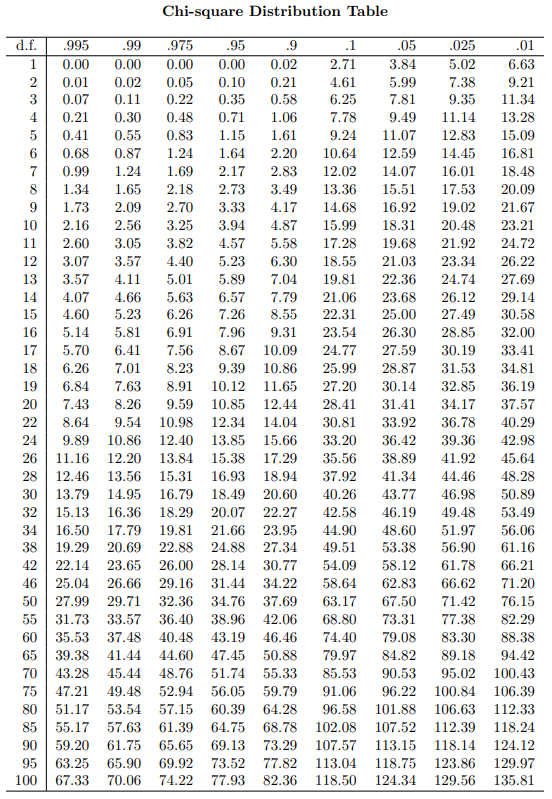
\includegraphics{chisquare.png}
\caption{Table containing the critical values of the chi-square distribution.}
\end{figure}

\hypertarget{example-14}{%
\subsubsection{Example}\label{example-14}}

Rock-scissors-paper is a game of chance in which any player should be expected to win, tie and lose with equal frequency. Over the course of 30 games a player could be expected to win approximately ten times, lose ten times and tie times. Imagine a random sample of 24 games:

\begin{longtable}[]{@{}rr@{}}
\caption{\label{tab:table011} Chi Square Goodness of Fit}\tabularnewline
\toprule
Outcome & Frequency (Observed) \\
\midrule
\endfirsthead
\toprule
Outcome & Frequency (Observed) \\
\midrule
\endhead
Win & 4 \\
Loss & 13 \\
Tie & 7 \\
\bottomrule
\end{longtable}

It doesn't seem like the outcomes occur with equal probability. It seems that the player is losing much more frequently than they win or tie.

A \(\chi^2\) goodness of fit test could be used to determine if the distribution of these outcomes disagrees with an even distribution. This is essentially a hypothesis test:

\(H_0\): All the outcomes have equal probability.

\(H_a\): The outcomes do not have equal probability.

Since it's expected that the player should win, lose and tie with equal frequency the expected outcomes are 8 wins, 8 losses and 8 ties.

\begin{longtable}[]{@{}rrr@{}}
\caption{\label{tab:table0011} Chi Square Goodness of Fit}\tabularnewline
\toprule
Outcome & Frequency (Observed) & Frequency (Expected) \\
\midrule
\endfirsthead
\toprule
Outcome & Frequency (Observed) & Frequency (Expected) \\
\midrule
\endhead
Win & 4 & 8 \\
Loss & 13 & 8 \\
Tie & 7 & 8 \\
\bottomrule
\end{longtable}

Calculating \(\chi^2\) gives:

\[\chi^2=\sum_{k=1}^{n}\frac{(O_k-E_k)^2}{E_k},\]

\[\chi^2=\frac{(4-8)^2}{8}+\frac{(13-8)^2}{8}+\frac{(7-8)^2}{8},\]
\[\chi^2=\frac{(-4)^2}{8}+\frac{(5)^2}{8}+\frac{(-1)^2}{8},\]
\[\chi^2=\frac{16}{8}+\frac{25}{8}+\frac{1}{8},\]

\[\chi^2=\frac{42}{8},\]

\[\chi^2=5.25.\]

After calculating \(chi^2\) the number of degrees of freedom, df, is needed. This is given by:

\[df=(p-1),\]

where p is the number of categories.

There are three categories (win, lose or tie) so the degrees of freedom, df, is given by:

\[df=(3-1)=2.\]
A \(\chi^2\) table is used to compare the calculated value of \(\chi^2\) with critical values that correspond to three degrees of freedom and a desired significance level.

For a \(df\) of 3 and a desired significance of 0.05 the calculated \(\chi^2\) value would need to be greater than 7.81 to reject the null hypothesis. In this case, \(\chi^2=5.25\) which is not greater than 7.81 so the null hypothesis is not rejected.

\hypertarget{chi-square-test-of-independence}{%
\subsection{Chi-Square Test of Independence}\label{chi-square-test-of-independence}}

The chi-square test of independence is used when two categorical variables are to be tested for independence. The aim is to analyze whether the characteristic values of the first variable are influenced by the characteristic values of the second variable and vice versa.

In order to calculate the chi-square, an observed and an expected frequency must be given. In the independence test, the expected frequency is the one that results when both variables are independent. If two variables are independent, the expected frequencies of the individual cells are obtained with:

\[\textrm{Expected Value}= \frac{\textrm{Row Total} \times \textrm{Column Total}}{\textrm{Grand Total}}.\]
Note that this differs from the goodness of fit test.

The calculation of degrees of freedom also differs and is given by:

\[df=(p-1)(q-1),\]

where p is the number of rows and q is the number of columns.

\hypertarget{example-15}{%
\subsubsection{Example}\label{example-15}}

The example below calculates chi square for some simulated data.

\begin{longtable}[]{@{}rrrr@{}}
\caption{\label{tab:table12} Educational Attainment: Observed Values}\tabularnewline
\toprule
Education & Male (Observed) & Female (Observed) & Total \\
\midrule
\endfirsthead
\toprule
Education & Male (Observed) & Female (Observed) & Total \\
\midrule
\endhead
GCSE & 15 & 13 & 28 \\
A Level & 5 & 3 & 8 \\
Total & 20 & 16 & 36 \\
\bottomrule
\end{longtable}

Expected values are calculated using:

\[\textrm{Expected Value}= \frac{\textrm{Row Total} \times \textrm{Column Total}}{\textrm{Grand Total}}.\]

The results are shown below:

\begin{longtable}[]{@{}rrr@{}}
\caption{\label{tab:table13} Educational Attainment: Expected Values}\tabularnewline
\toprule
Education & Male (Expected) & Female (Expected) \\
\midrule
\endfirsthead
\toprule
Education & Male (Expected) & Female (Expected) \\
\midrule
\endhead
GCSE & 16 & 12 \\
A Level & 4 & 4 \\
\bottomrule
\end{longtable}

Now calculate \(\chi^2\):

\[\chi^2=(15-16)^2/16 +(13-12)^2/12+(5-4)^2/4 + (3-4)^2/4 = 0.645.\]

After calculating \(\chi^2\) the degrees of freedom, df, is needed. This is given by:

\[df=(p-1)(q-1)=(2-1)(2-1)=1.\]

For a significance level of 5\% a \(\chi^2\) value greater than 3.84 is needed. Since the calculated \(\chi^2\) value is larger, there is a significant difference and the null hypothesis is rejected. A p value close to zero means that our variables are very unlikely to be completely unassociated in some population. However, this does not mean the variables are strongly associated; a weak association in a large sample size may also result in p\textless0.05.

\hypertarget{strength-of-association}{%
\section{Strength of Association}\label{strength-of-association}}

A few different statistics can be used for calculating effect size when a Chi squared test has been conducted, depending on the number of categories for each variable, the type of variables (nominal or ordinal) and the nature of the study.

\hypertarget{phi}{%
\subsection{Phi}\label{phi}}

In the case where there are only two categories for each variable, then effect size can be measured using phi (\(\phi\)). Phi is a measure for the strength of an association between two categorical variables in a 2 \(\times\) 2 contingency table. It is calculated by taking the chi-square value, dividing it by the sample size, and then taking the square root of this value \citep{akoglu}.

This is calculated using the Chi-square value (\(\chi^2\)) and the sample size (\(n\)), as follows:

\[\phi=\sqrt{\frac{\chi^2}{n}}.\]

In our case:

\[\phi=\sqrt{\frac{0.3125}{36}}=0.13.\]

This is considered a small effect (0.1 is considered a small effect size, 0.3 medium and 0.5 and above large).

Note also that an extension of ϕ for nominal variables with more than two categories is Cramer's V, while other measures of effect size include relative risk and odds ratio.

\hypertarget{cramers-v}{%
\subsection{Cramer's V}\label{cramers-v}}

Cramer's V is an alternative to phi in tables bigger than 2 \(\times\) 2 tabules \citep{akoglu}.

\[V = \sqrt{\frac{\chi^2}{n*min(r-1,c-1)}},\]

where \(n\) in the sample size and \(min()\) is the minimum of the two arguments \(r-1\) and \(c-1\). A Cramer's V value of 0-0.29 indicates a weak association; 0.3-0.59 indicates a moderate association and a Cramer's V of 0.6-1 indicates a strong association. The scale goes from complete independence to perfect association.

Association should never be greater than 1. A relatively weak correlation is all that can be expected when a phenomena is only partially dependent on the independent variable.

An alternative association measure for two nominal variables is the contingency coefficient. However, it's better avoided since its maximum value depends on the dimensions of the contingency table involved.

For two ordinal variables, a Spearman correlation or Kendall's tau are preferable over Cramér's V. For two metric (interval or ratio) variables, a Pearson correlation is the preferred measure.

\hypertarget{relative-risk}{%
\section{Relative Risk}\label{relative-risk}}

The relative risk (RR) and the odds ratio (OR) are widely used in medical research and are very commonly used measures of association in epidemiology \citep{schmidtty}. Relative risk is a comparison of the chance of an event happening in one group to the chance of it happening in another. For instance, the relative risk of lung cancer in smokers compared to non-smokers is the chance of getting lung cancer for smokers divided by the chance for non-smokers \citep{tenny}. Relative risk only shows the difference in likelihood between the two groups, it does not show the actual risk of the event happening \citep{tenny}.

The Relative Risk is used when comparing the probability of an event occurring to all possible events considered in a study.

For example consider the risk of developing cancer in those exposed and unexposed to second hand smoke. On a study's conclusion we might have a table like the one below:

\begin{longtable}[]{@{}rrr@{}}
\caption{\label{tab:table14}}\tabularnewline
\toprule
Status & Disease & No Disease \\
\midrule
\endfirsthead
\toprule
Status & Disease & No Disease \\
\midrule
\endhead
Exposed & A & B \\
Unexposed & C & D \\
\bottomrule
\end{longtable}

To calculate the relative risk associated with an exposure we must compare the risk (incidence) among the exposed to those not exposed.

\[\textrm{Ratio of Risks} = \frac{\textrm{Disease Risk (incidence) in exposed (A/(A+B))}}{ \textrm{Disease Risk (incidence) in Non-Exposed (C/(C+D))}} = \textrm{Relative Risk}. \]

Let's add values to do the calculations:

\begin{longtable}[]{@{}rrr@{}}
\caption{\label{tab:table15}}\tabularnewline
\toprule
Status & Disease & No Disease \\
\midrule
\endfirsthead
\toprule
Status & Disease & No Disease \\
\midrule
\endhead
Exposed & A & B \\
Unexposed & C & D \\
\bottomrule
\end{longtable}

\[\textrm{Disease Risk (incidence) in exposed}=\frac{366}{366+32}=0.92,\]
\[\textrm{Disease Risk (incidence) in unexposed}=\frac{64}{64+319}=0.17,\]

\[\textrm{Relative Risk}=\frac{0.92}{0.17}=5.41.\]
RR=1, the incidence in the exposed is the same as the incidence in the non-exposed. No increased risk, no association.

RR\textgreater1, the incidence in the exposed is greater than the incidence in the non-exposed. Increased risk, positive association.

RR\textless1, the incidence in the exposed is lower than the incidence in the non exposed. Decreased risk, negative association.

The further the RR is from 1 the stronger the association.

The relative risk will be reported alongside a p value or a 95\% confidence interval. If the p value is not less than 0.05 or if the confidence interval includes 1 then the RR is not statistically significant.

Information

You cannot calculate relative risk in a case control study. For instance, a study might involve a control group of 100 people without cancer and a group of 100 people with cancer. The disease rate might be 50\% because of how the study was designed.

\hypertarget{odds-ratio}{%
\section{Odds Ratio}\label{odds-ratio}}

The odds ratio is used in cohort or case-control studies.

Information

Odds ratios consistently overestimate risk.

Odds are not the same as probability:

\[\textrm{Odds}=\frac{\textrm{Probability}}{1-\textrm{Probability}}.\]

For instance, a 60\% probability to win gives 1.5 odds to win.

Given some data:

\begin{longtable}[]{@{}rrr@{}}
\caption{\label{tab:table16}}\tabularnewline
\toprule
Status & Disease (case) & Disease (Control \\
\midrule
\endfirsthead
\toprule
Status & Disease (case) & Disease (Control \\
\midrule
\endhead
Exposed & A & B \\
Unexposed & C & D \\
\bottomrule
\end{longtable}

The Odds ratio is given by:

\[\textrm{Odds Ratio} = \frac{\textrm{odds that a case was exposed (A/C)}}{\textrm{odds that a control was exposed (B/D)}}.\]

Here's an example with real data:

\begin{longtable}[]{@{}
  >{\raggedleft\arraybackslash}p{(\columnwidth - 4\tabcolsep) * \real{0.3333}}
  >{\raggedleft\arraybackslash}p{(\columnwidth - 4\tabcolsep) * \real{0.3333}}
  >{\raggedleft\arraybackslash}p{(\columnwidth - 4\tabcolsep) * \real{0.3333}}@{}}
\caption{\label{tab:table17}}\tabularnewline
\toprule
\begin{minipage}[b]{\linewidth}\raggedleft
Exposure: Parental smoking in pregnancy
\end{minipage} & \begin{minipage}[b]{\linewidth}\raggedleft
Disease (Cancer)
\end{minipage} & \begin{minipage}[b]{\linewidth}\raggedleft
No Disease (No Cancer)
\end{minipage} \\
\midrule
\endfirsthead
\toprule
\begin{minipage}[b]{\linewidth}\raggedleft
Exposure: Parental smoking in pregnancy
\end{minipage} & \begin{minipage}[b]{\linewidth}\raggedleft
Disease (Cancer)
\end{minipage} & \begin{minipage}[b]{\linewidth}\raggedleft
No Disease (No Cancer)
\end{minipage} \\
\midrule
\endhead
Yes: Smoking & 87 & 147 \\
No: Non-Smoking & 201 & 508 \\
\bottomrule
\end{longtable}

The odds ratio is:

\[OR=\frac{(\frac{87}{201})}{(\frac{147}{508})}=1.48.\]
This is different from the relative risk equation.

OR = 1, exposure is not associated with the disease.

OR \textgreater{} 1, exposure is positively associated with the disease.

OR \textless{} 1, exposure is negatively associated with the disease.

The further the OR is from 1, the stronger the association.

\hypertarget{chi-square-homogeneity-test}{%
\section{Chi Square Homogeneity Test}\label{chi-square-homogeneity-test}}

The Chi-square homogeneity test can be used to check whether two or more samples come from the same population. One question could be whether the subscription frequency of three fictional video streaming services Netflocks, Amazing, Fizzney and Tantamount differ in different age groups. As a fictitious example, a survey is made in three age groups with the following result:

\begin{longtable}[]{@{}rrrr@{}}
\caption{\label{tab:table18}}\tabularnewline
\toprule
Network & 15-25 & 25-35 & 35-45 \\
\midrule
\endfirsthead
\toprule
Network & 15-25 & 25-35 & 35-45 \\
\midrule
\endhead
Netflocks & 25 & 23 & 20 \\
Amazing & 29 & 30 & 33 \\
Fizzney & 11 & 13 & 12 \\
Tantamount & 16 & 24 & 26 \\
\bottomrule
\end{longtable}

As with the chi-square independence test, this result is compared with the table that would result if the distributions of Streaming providers were independent of age.

The process is the same as in the Independence test where the expected values are calculated.

Summary

\textbf{Goodness-of-fit}

Use the goodness-of-fit test to decide whether a population with an unknown distribution ``fits'' a known distribution.

\(H_0\): The population fits the given distribution.

\(H_a\): The population does not fit the given distribution.

\textbf{Independence}

Use the test for independence to decide whether two variables (factors) are independent or dependent.

\(H_0\): The two variables (factors) are independent.

\(H_a\): The two variables (factors) are dependent.

\textbf{Homogeneity}

Use the test for homogeneity to decide if two or more populations with unknown distributions have the same distribution as each other.

\(H_0\): The two populations follow the same distribution.

\(H_a\): The two populations have different distributions.

\hypertarget{datvis}{%
\chapter{Data Visualisation}\label{datvis}}

\begin{center}\rule{0.5\linewidth}{0.5pt}\end{center}

\hypertarget{data-visualisation}{%
\section{Data Visualisation}\label{data-visualisation}}

Data visualisation is formally defined as the encoding of data using visual cues such as variations in the size, shape and colour of geometric objects (points, lines, bars). The encoding is generally informed by the relationships within the data.

The bar chart below shows the marital status of people in Northern Ireland based on the Census 2011 data \citep{census2011}. The frequencies of different marital statuses have been mapped to the heights of the bars.

\hypertarget{visual-cues}{%
\section{Visual Cues}\label{visual-cues}}

Whether data is visualised using points, lines, bars or something else entirely is largely determined by the relationships within the data. Some of the visual cues and relationships used to inform data visualisation are shown below.

The illustration above shows some of the visual cues used to encode data. Magnitudes are typically mapped to sizes of objects. Colour is often used to represent quantities or highlight data. Shapes can be used to represent qualitative data.

\hypertarget{relationships-in-data}{%
\section{Relationships in Data}\label{relationships-in-data}}

The \href{https://analysisfunction.civilservice.gov.uk/policy-store/data-visualisation-charts/\#section-9}{Government Statistical Service} has produced guidance on the relationships in data and how they inform chart choices. The guidance can be useful and some of the key points are summarised below.

\hypertarget{frequency-distributions}{%
\subsection{Frequency Distributions}\label{frequency-distributions}}

Histograms and bar charts are useful for showing category frequencies. Population by age band for instance could be visualised using a histogram or bar chart. A boxplot can also be useful in visualising additional descriptive statistics such as the mean, median, quartiles, outliers and the range.

The figure below shows the age distributions of GPs in Northern Ireland as of 2020 \citep{family}.

\hypertarget{time-series}{%
\subsection{Time Series}\label{time-series}}

A line chart is often used to demonstrate the trend of a variable over some time period. For instance, temperature over time can be visualised with a line chart.

The line chart below shows simulated temperature data for Northern Ireland.

\hypertarget{rankings}{%
\subsection{Rankings}\label{rankings}}

Data that is ranked usually consists of categories presented in ascending or descending order. A bar chart may be used to show the comparisons between the different categories. Sometimes, change in ranking over time is shown through slope charts but usually only when comparing a start date and an end date without consideration for the time period in between.

The slope chart below shows the change in the percentage of Health Survey respondents reporting a longstanding illness between 2010 and 2020 \citep{health}.

\hypertarget{deviation}{%
\subsection{Deviation}\label{deviation}}

Deviation from a reference value can be shown through bar charts.

\hypertarget{correlation}{%
\subsection{Correlation}\label{correlation}}

Correlation is usually visualised using scatterplots. Scatterplots are a good way to show comparisons between observations of two variables to determine if there is some correlation because it quickly becomes apparent if there is correlation between the variables or not.

The scatterplot below shows simulated height and weight data.

\hypertarget{magnitude}{%
\subsection{Magnitude}\label{magnitude}}

Comparing differences in the magnitudes of values often relies on bar charts. Comparing the total number of research papers by journal for insance.

\hypertarget{spatial}{%
\subsection{Spatial}\label{spatial}}

Cartograms and heat mapping are common ways to show differences between geographical regions.

\hypertarget{why-visualise-data}{%
\section{Why Visualise Data?}\label{why-visualise-data}}

In general, people are better at recognising differences in shapes, colours and sizes than they are at identifying the number of times a value occurs or the differences between values in a large excel spread sheet. For this reason data visualisation can be used to find errors in data quickly. It's much easier to recognise an anomalous value on a bar chart than in an Excel spread sheet. Data visualisation can also be used to see patterns that are difficult to determine by looking at raw data.
Data visualisation can also be used to:

\begin{itemize}
\tightlist
\item
  Answer research questions.
\item
  Discover new research questions.
\item
  Explain complex relationships in data visually.
\item
  Aid in decision making.
\item
  Engage and inform.
\end{itemize}

\hypertarget{data-visualisation-tools}{%
\section{Data Visualisation Tools}\label{data-visualisation-tools}}

New programming languages and software products have made data analysis and visualisation vastly more accessible. In addition, many of these facilitate dynamic or interactable visualisations. There is an ever expanding ecosystem of data visualisation tools (many of which have been used in this document) including:

\begin{itemize}
\tightlist
\item
  \textbf{Excel} and \textbf{SPSS} produce high quality visualisations and while dynamic visuals are not their focus they are often the simplest and most time efficient option for visualising data.
\item
  \textbf{Genially} is an online tool for creating interactive and animated content that is particularly effective for presentations.
\item
  \textbf{Tableau} and \textbf{Power BI} are visual analytics platforms which are well suited to the development of dashboards to visualise complex interconnected data sets.
\item
  \textbf{Flourish} can be used to produce interactive visuals although its functionality is more limited than Power BI or Tableau. It can be useful for animated visuals however it struggles with larger data sets.
\item
  \textbf{Javascript} facilitates data visualisation through its D3 library. D3 has a steep learning curve as it requires JavaScript skills to use it effectively however it offers a greater degree of customisation and a broader spectrum of visualisation options as a result.
\item
  \textbf{Python} libraries such as Matplotlib, Seaborn and Plotly can also be used to visualise data. The learning curve is steep as it requires programming skills to use Python effectively however Python offers customisation options that are not available in Excel or Power BI. Python has been used to produce many of the visuals in this e-book.
\item
  \textbf{R} is another useful tool with libraries such as ggplot2 which can be used to visualise data. This is the programming language used to write this e-book.
\end{itemize}

\hypertarget{dynamic-visualisations-dashboards}{%
\section{Dynamic Visualisations (Dashboards)}\label{dynamic-visualisations-dashboards}}

There are a number of considerations when developing dynamic data visualisations (sometimes called dashboards) as not all data visualisations need to be dynamic.

Considering the audience, objectives and what visuals will be most appropriate to communicate data can help in determining whether a dynamic or interactive visualisation is needed.

Dashboard style visualisations are best suited to data reporting where there is a need to repeatedly produce the same visuals or reports either daily, monthly, quarterly or annually.

Power BI is well designed for these types of visualisation requirements as it offers automation options enabling data sets to be refreshed at regular time intervals.
Automation can be as simple as setting a refresh time in the Power BI dashboard and manually updating the excel file it stores in memory or it can be more complex and involve using programming languages to make API calls and perform automated calculations.

Producing dynamic visualisations is often considerably more time expensive than producing static visuals and time constraints should be considered before developing a dashboard visualisation.

\hypertarget{best-practice}{%
\subsection{Best Practice}\label{best-practice}}

GSS have produced \href{https://gss.civilservice.gov.uk/policy-store/top-tips-for-designing-dashboards/}{guidance on designing dashboards} that covers most aspects of dashboard design. The content below summarises some of the key points in this guidance.

\textbf{Consider Audience and User Needs}

Consider the user needs and whether a dashboard is really needed. Often the simplest solution (bar charts drawn in Excel or SPSS) is the best. Consider the visuals used and whether they're the best way to communicate the data. Sometimes tables or even text can communicate data better than a visual.

\textbf{Guidance}

Providing guidance on how to use a dynamic visual or dashboard is important as many users will not be familiar with interactive dashboards. Guidance can be provided through supplementary documentation, blog text if the visual is being embedded, or it can be provided through tool tips and information pages in the dashboard itself.

\textbf{Streamline Content}

When adding any new data or visuals it is important to ask whether it adds value. Try to group related content and streamlining the content to guide the users through the data.

\textbf{Automate }

Automation can be simple or complex, it can be achieved by setting a refresh date in a Power BI dashboard. It can also involve the use of programming languages to make API calls, web scrape data and perform calculations. Automation typically results in less manual updating and a reduced chance of error and can make the management of the product less resource intensive. It's important to note that automation does not necessarily mean less work, the scripts used to automate processes will need to be updated as languages are developed and updated over time.

\textbf{Consider Design Principles}

Give your dashboard a header and dedicated areas for visuals. Consider other dashboards you have seen in the past and draw inspiration from web design. Most websites have a navigation bar at the top, lists with filters along the left or right hand side and content in the center of the page. Think about things like symmetry, flow and a consistent style or layout. Use white space where possible and try to avoid cluttered visualisations.

\textbf{Ensure Accessibility}

Ensure your product is accessible by checking the colour contrast ratios of text and including alt text in your visualisations where possible. Ensure the fonts are large enough to read and avoid using multiple fonts.

  \bibliography{example.bib}

\end{document}
